\documentclass[a4paper,11pt]{article}

\usepackage[portuguese]{babel}
\usepackage[utf8]{inputenc}
\usepackage{amsmath}
\usepackage{graphicx}
\usepackage{hyperref}
\usepackage{float}
\usepackage{subfig}
\usepackage{fixltx2e}
\usepackage[bottom]{footmisc}
\usepackage{listings}
\usepackage{xargs}                      % Use more than one optional parameter in a new commands
\usepackage[usenames,table,x11names,svgnames,dvipsnames,pdftex]{xcolor}
\usepackage[colorinlistoftodos,prependcaption,textsize=tiny]{todonotes}
\newcommandx{\unsure}[2][1=]{\todo[linecolor=red,backgroundcolor=red!25,bordercolor=red,#1]{#2}}
\newcommandx{\change}[2][1=]{\todo[linecolor=blue,backgroundcolor=blue!25,bordercolor=blue,#1]{#2}}
\newcommandx{\info}[2][1=]{\todo[linecolor=OliveGreen,backgroundcolor=OliveGreen!25,bordercolor=OliveGreen,#1]{#2}}
\newcommandx{\improvement}[2][1=]{\todo[linecolor=Plum,backgroundcolor=Plum!25,bordercolor=Plum,#1]{#2}}
\newcommandx{\thiswillnotshow}[2][1=]{\todo[disable,#1]{#2}}
\usepackage[font=footnotesize]{caption}
\usepackage[hypcap]{caption}
\usepackage[top=2.5cm, bottom=2.5cm, left=2.5cm, right=2.5cm]{geometry}
\usepackage{enumerate}
\usepackage[siunitx,american]{circuitikz}

\setcounter{tocdepth}{3}
\setcounter{secnumdepth}{4}

\numberwithin{equation}{section}
\addto\captionsportuguese{\renewcommand{\contentsname}{Índice}}

\linespread{1.3}
\usepackage{indentfirst}

\begin{document}
\begin{titlepage}
\begin{center}

\hfill \break
\hfill \break


\includegraphics[width=0.3\textwidth]{img/logo}~\\[1cm] 

\textsc{\LARGE Instituto Superior Técnico}\\[0.25cm]
\textsc{\Large Mestrado Integrado em Engenharia Electrotécnica e de Computadores}\\[1.8cm]
\textsc{\huge Electrónica de Potência}\\[0.25cm]

\vspace{6mm}

{\huge \bfseries Conversor CA/CC Monofásico \linebreak Comandado de Onda Completa \\[0.7cm]}
{\bfseries Rectificador de onda completa totalmente comandado e semi-comandado \\[1cm]}

\begin{tabular}{ l l }
	João Bernardo Sequeira de Sá & \hspace{2mm} n.º 68254 \\
	Maria Margarida Dias dos Reis & \hspace{2mm} n.º 73099 \\
	Rafael Augusto Maleno Charrama Gonçalves & \hspace{2mm} n.º 73786 \\
	Nuno Miguel Rodrigues Machado & \hspace{2mm} n.º 74236
\end{tabular}

\vspace{7mm}

Turno de Segunda-feira das 17h00 - 20h00

\vfill

{\large Lisboa,  de Novembro de 2015} 
	
\end{center}
\end{titlepage}
	
\tableofcontents
\pagebreak

\section{Introdução}

Este trabalho laboratorial é uma continuação do trabalho 2A em que se estudou o conversor CA/CC (rectificador) de meia onda comandado e semi-comandado monofásico. Desta vez o objetivo é compreender o funcionamento do rectificador monofásico comandado de onda completa.

Este trabalho está separado em duas partes; na primeira estuda-se o funcionamento do conversor totalmente comandado e na segunda o semi-comandado.

Aquilo que distingue o rectificador de onda completa do de meia onda é a presença de 4 tiristores, tal como pode ser observado na \autoref{fig:circuit_1}, em oposição a apenas 1 tiristor como se tinha no rectificador de meia onda.


\begin{figure}[h]
	\centering
	%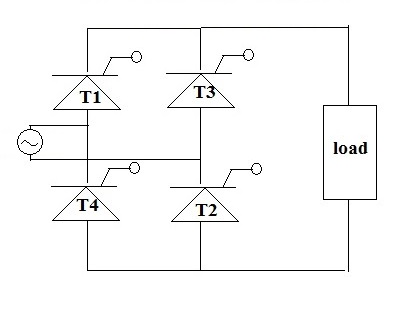
\includegraphics[keepaspectratio=true, scale=0.8]{img/circuito}
	\begin{tikzpicture}[scale=0.7, transform shape]
	\draw
		(0,0) node[] (origin) {} to[sV] ++(0,2) node[] (source) {}
		(origin) to[short,-*] ++ (5,0) to[short] ++ (0,2) to[Ty,l_=$T3$,-*] ++ (0,2) to[short] ++ (2,0) to[generic,l=Carga] ++ (0,-6) to[short] ++ (-2,0) node[] (bottomty) {} to[short] ++(-2,0) to[Ty, l_=$T4$] ++ (0,2) to[short,-*] ++ (0,2) node[] (topty) {} to[short] (source)
		(bottomty) to[Ty,l_=$T2$,*-*] ++ (0,2)
		(topty) to[Ty,l_=$T1$] ++(0,2) to[short] ++ (2,0)
		;
	\end{tikzpicture}
	\caption{Esquema do rectificador de onda completa monofásico comandado.}
	\label{fig:circuit_1}
	\vspace{-0.8em}
\end{figure}

O funcionamento desta topologia depende de qual o par de tiristores que está a conduzir a uma dada altura. Fazendo uso da nomenclatura da \autoref{fig:circuit_1} observa-se que T1 e T2 podem ser disparados durante a alternância positiva da tensão de entrada, sendo que T4 e T3 podem ser disparados durante a alternância negativa \cite{Silva}. Para o primeiro caso tem-se que o ângulo de disparo, $\alpha$, pode variar entre $0$ e $\pi$ onde para o segundo caso se faz uso de $\alpha + \pi$. Tal como já foi visto no trabalho anterior a altura em que um tiristor entra ao corte depende do momento em que a corrente aos terminais deste passa por zero, pelo que o funcionamento para uma carga puramente resistiva difere do de uma carga indutiva.

Espera-se assim que as formas de onda para a tensão e corrente numa carga indutiva seja tal como se vê na \autoref{fig:andamento}.

\begin{figure}[h]
	\centering
	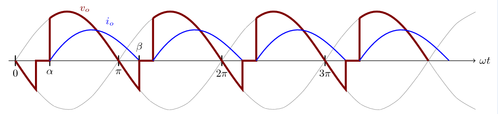
\includegraphics[keepaspectratio=true, scale=0.8]{img/andamento}
	\caption{Formas de onda para carga indutiva.}
	\label{fig:andamento}
	\vspace{-0.8em}
\end{figure}

O resultado é que, ao contrário do rectificador de meia onda, tanto para a alternância positiva da tensão de entrada, como para a negativa, se irá ter corrente na carga; obtém-se um comportamento desta corrente muito mais próximo do continuo e um conteúdo harmónico substancialmente inferior. Observa-se também que devido a isto, o valor médio da corrente na entrada será zero.

Para a segunda parte do trabalho tem-se um rectificador semi-comandado, onde se substitui dois dos rectificadores por dois díodos. Isto pode ser feito caso a carga não exija inversão da tensão aos seus terminais, sendo neste caso imposição da topologia que a tensão de saída tenha sempre o mesmo sinal, devido à presença dos díodos.


\section{Condução do Trabalho}

\subsection{Rectificador de onda completa totalmente comandado}


\subsubsection{Carga resistiva pura (R)}

De maneira a analisar o funcionamento do circuito com cargas resistivas, foi ligado à saída do Rectificador de Onda Completa controlado um reóstato.


\paragraph{Formas de onda da tensão e corrente na entrada} \mbox{}\

Inicialmente, observou-se a forma de onda da tensão e da corrente na entrada do circuito.

\begin{figure}[H]
	\centering
	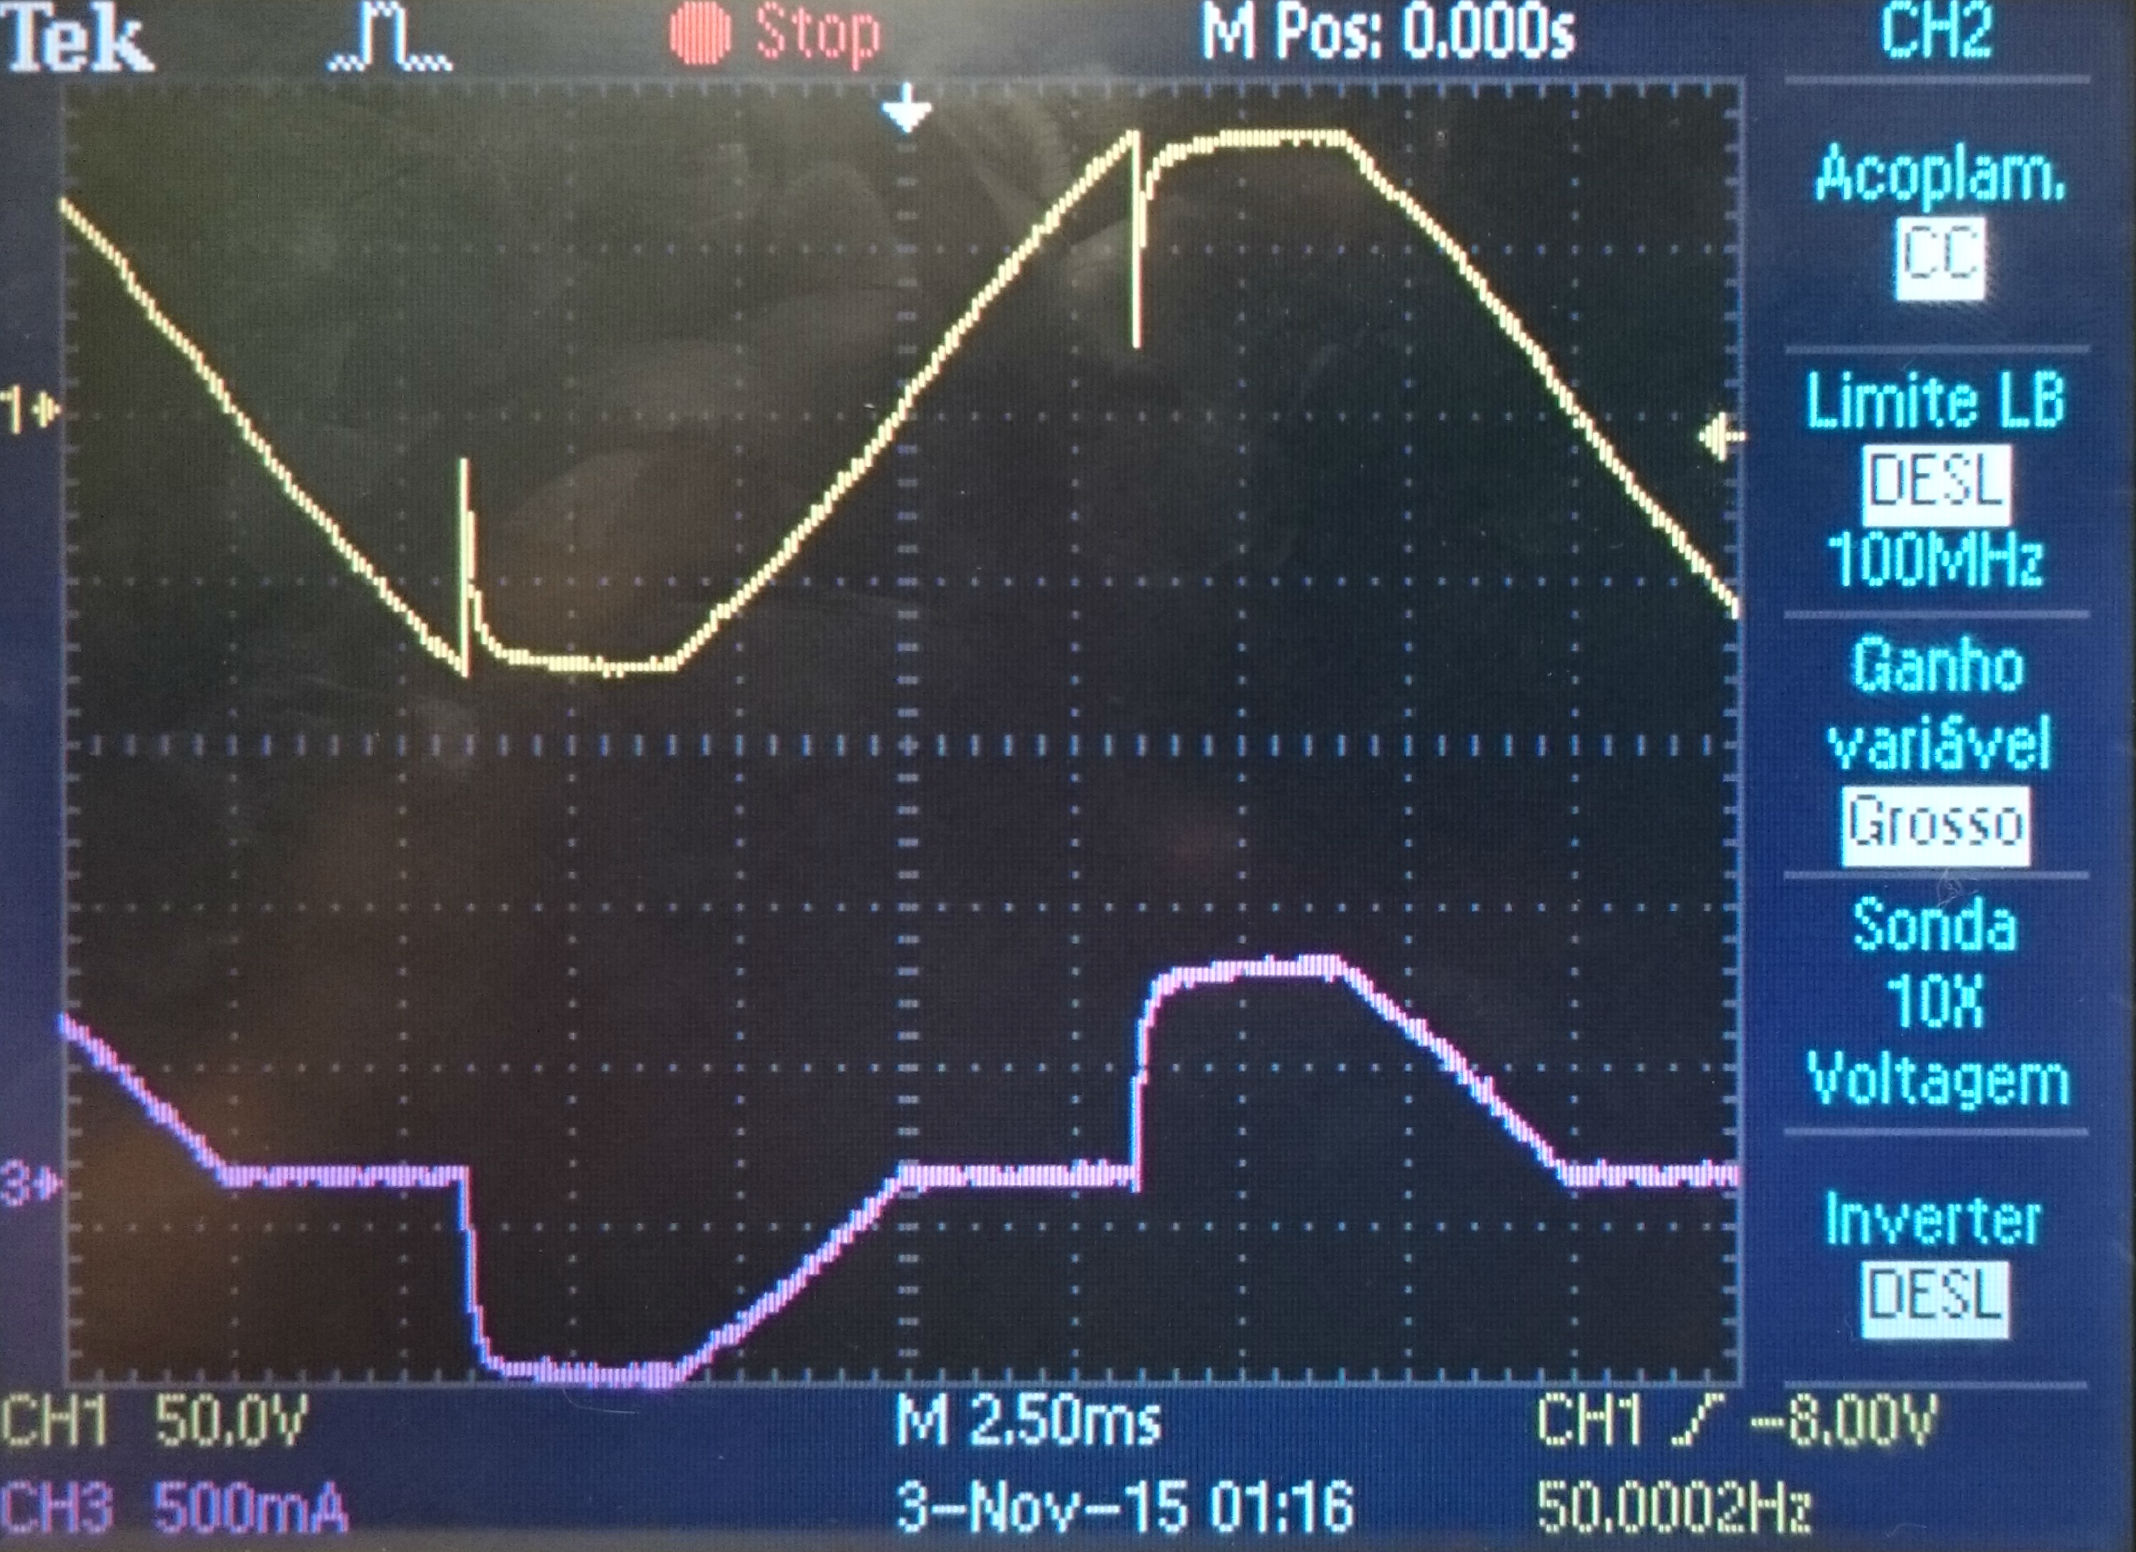
\includegraphics[keepaspectratio=true, scale=0.12]{img/DSC_0181}
	\caption{Tensão (a amarelo) e corrente (a rosa) na entrada.}
	\label{fig:tcentrada}
	\vspace{-0.8em}
\end{figure}

Na \autoref{fig:tcentrada} observam-se quedas de tensão na entrada sempre que tirístores entram à condução. 

Como a carga é resistiva, a corrente é proporcional à tensão. Quando a tensão de entrada se anula, a corrente anula-se e os dispositivos que estão a conduzir passam ao corte. Como os tirístores complementares não são imediatamente activados ($\alpha > 0$), a corrente mantém-se a zero até ao disparo.

\paragraph{Formas de onda da tensão e corrente na carga} \mbox{}\

Na carga é possível observar a rectificação da onda completa, e as características resistivas da mesma.

\begin{figure}[H]
	\centering
	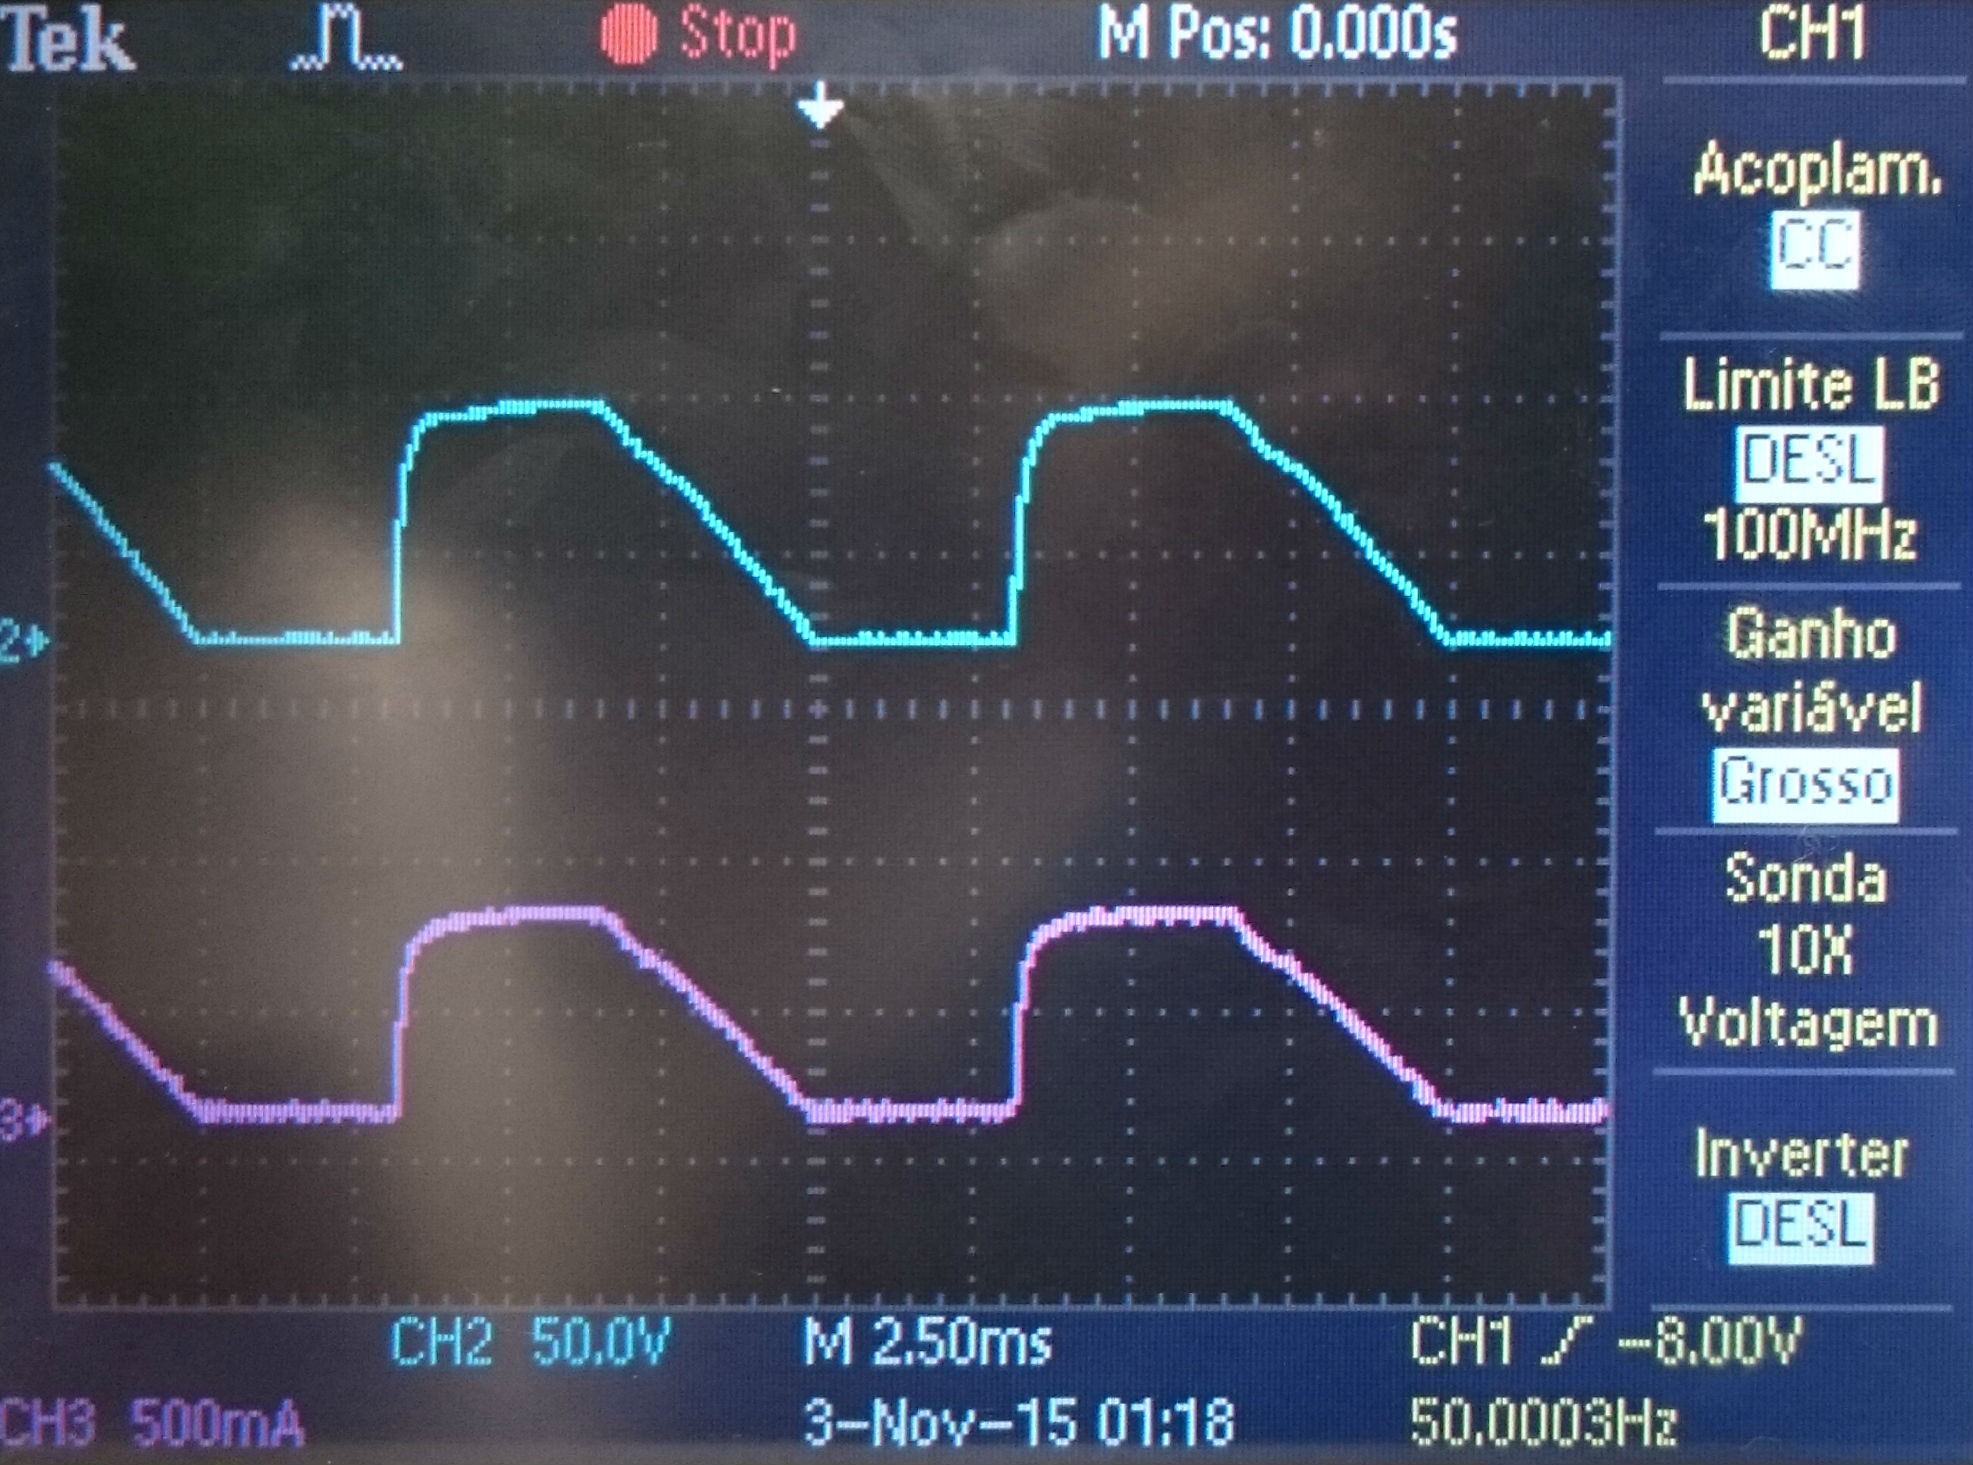
\includegraphics[keepaspectratio=true, scale=0.13]{img/DSC_0182}
	\caption{Tensão (a azul) e corrente (a rosa) na carga.}
	\label{fig:tccarga}
	\vspace{-0.8em}
\end{figure}

\paragraph{Formas de onda da tensão e corrente no tiristor} \mbox{}\

Cada par de tirístores conduz alternadamente com o par complementar.

\begin{figure}[H]
	\centering
	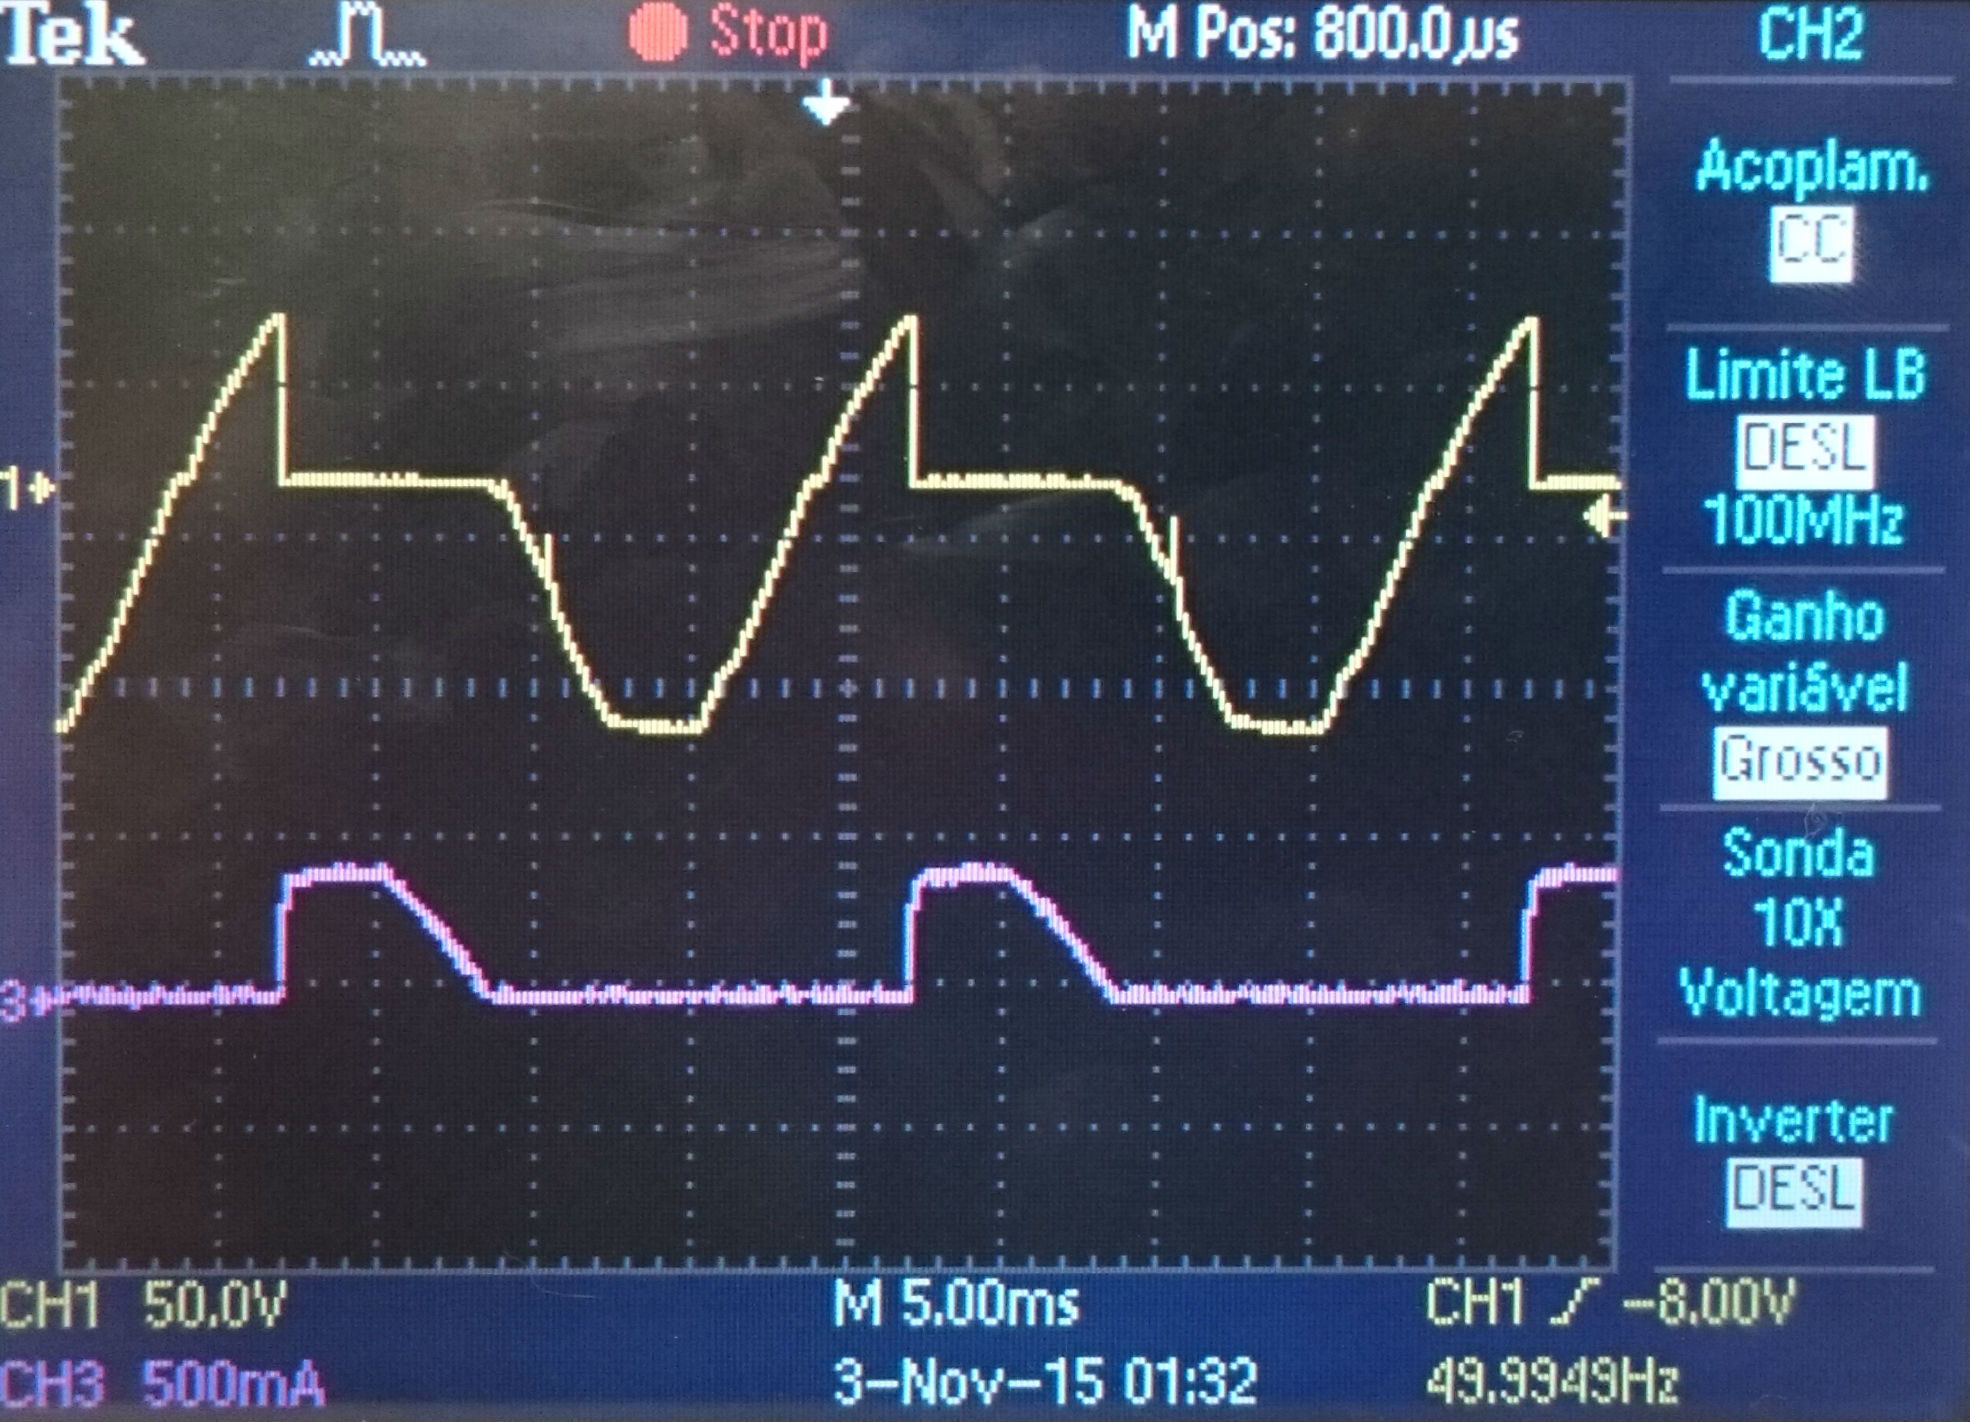
\includegraphics[keepaspectratio=true, scale=0.13]{img/DSC_0183}
	\caption{Tensão (a amarelo) e corrente (a rosa) no tiristor.}
	\label{fig:tctiristor}
	\vspace{-0.8em}
\end{figure}

Na \autoref{fig:tctiristor} observa-se a parte da corrente da carga que corresponde ao tirístor em questão, sendo que durante a condução, o tirístor está em curto-circuito.

Quando o dispositivo passa ao corte, cai sobre si toda a tensão de entrada.

\paragraph{Característica de comando do conversor} \mbox{}\

De maneira a calcular uma previsão teórica do valor médio da tensão de saída, foi utilizada a \autoref{eq:comandado_tensao}.

\begin{equation}
\label{eq:comandado_tensao}
\overline{v_O}=\frac{1}{\pi} \int_\alpha^\pi \sqrt{2} V \,\sin{(\omega t)}\;\mathrm{d}\omega t = \frac{\sqrt{2}V}{\pi}(1 + \cos{(\alpha)})
\end{equation}

\begin{table}[H]
\centering
\begin{tabular}{c c c c c c c}
\hfil & Ângulo de Disparo $[^\circ]$ & \hfil & $V_O\;[V]$ (teórico) & \hfil & $V_O\;[V]$ (experimental) & \hfil \\
\hline
			&$0$&	&$45$&		&$48$&\\
\rowcolor{SkyBlue}	&$30$&	&$42$&		&$46.2$&\\
			&$60$&	&$33.8$&	&$37.9$&\\
\rowcolor{SkyBlue}	&$90$&	&$22.5$&	&$25.6$&\\
			&$120$&	&$11.25$&	&$12.8$&\\
\rowcolor{SkyBlue}	&$150$&	&$3.02$&	&$1.48$&\\
\hline
\end{tabular}
\caption{Valor médio da tensão de saída em função do ângulo de disparo($V_i = 50 V$)}
\label{tab:akpk}
\end{table}

\begin{figure}[H]
	\centering
	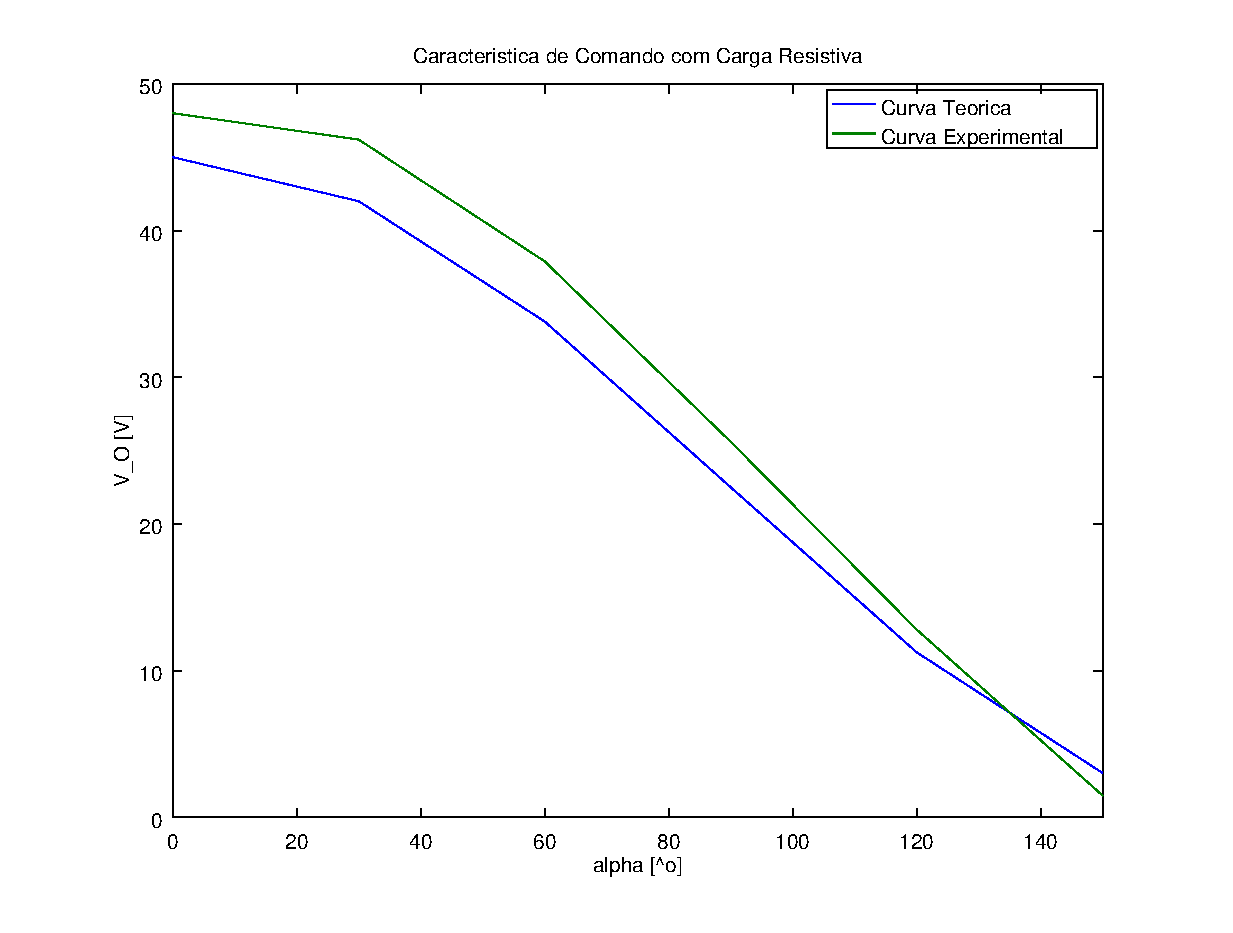
\includegraphics[keepaspectratio=true, width=0.8\textwidth]{img/comando1}
	\caption{Características teórica e experimental}
	\label{fig:comando1}
	\vspace{-0.8em}
\end{figure}

Um dos motivos pelos quais há diferenças entre os valores teóricos e os valores medidos é a deformação do sinal de entrada, que está longe de ser uma sinusóide.

\subsubsection{Carga indutiva RL}

\paragraph{Formas de onda da tensão e corrente na carga para funcionamento lacunar} \mbox{}\

Quando a carga tem uma componente indutiva substancial (na realidade, qualquer porção de circuito constitui uma espira, e portanto tem uma indutância, sendo que na maioria dos casos esta indutância é desprezável), a corrente passa a ter uma inércia associada, isto é, torna-se numa variável de estado.

\begin{figure}[H]
	\centering
	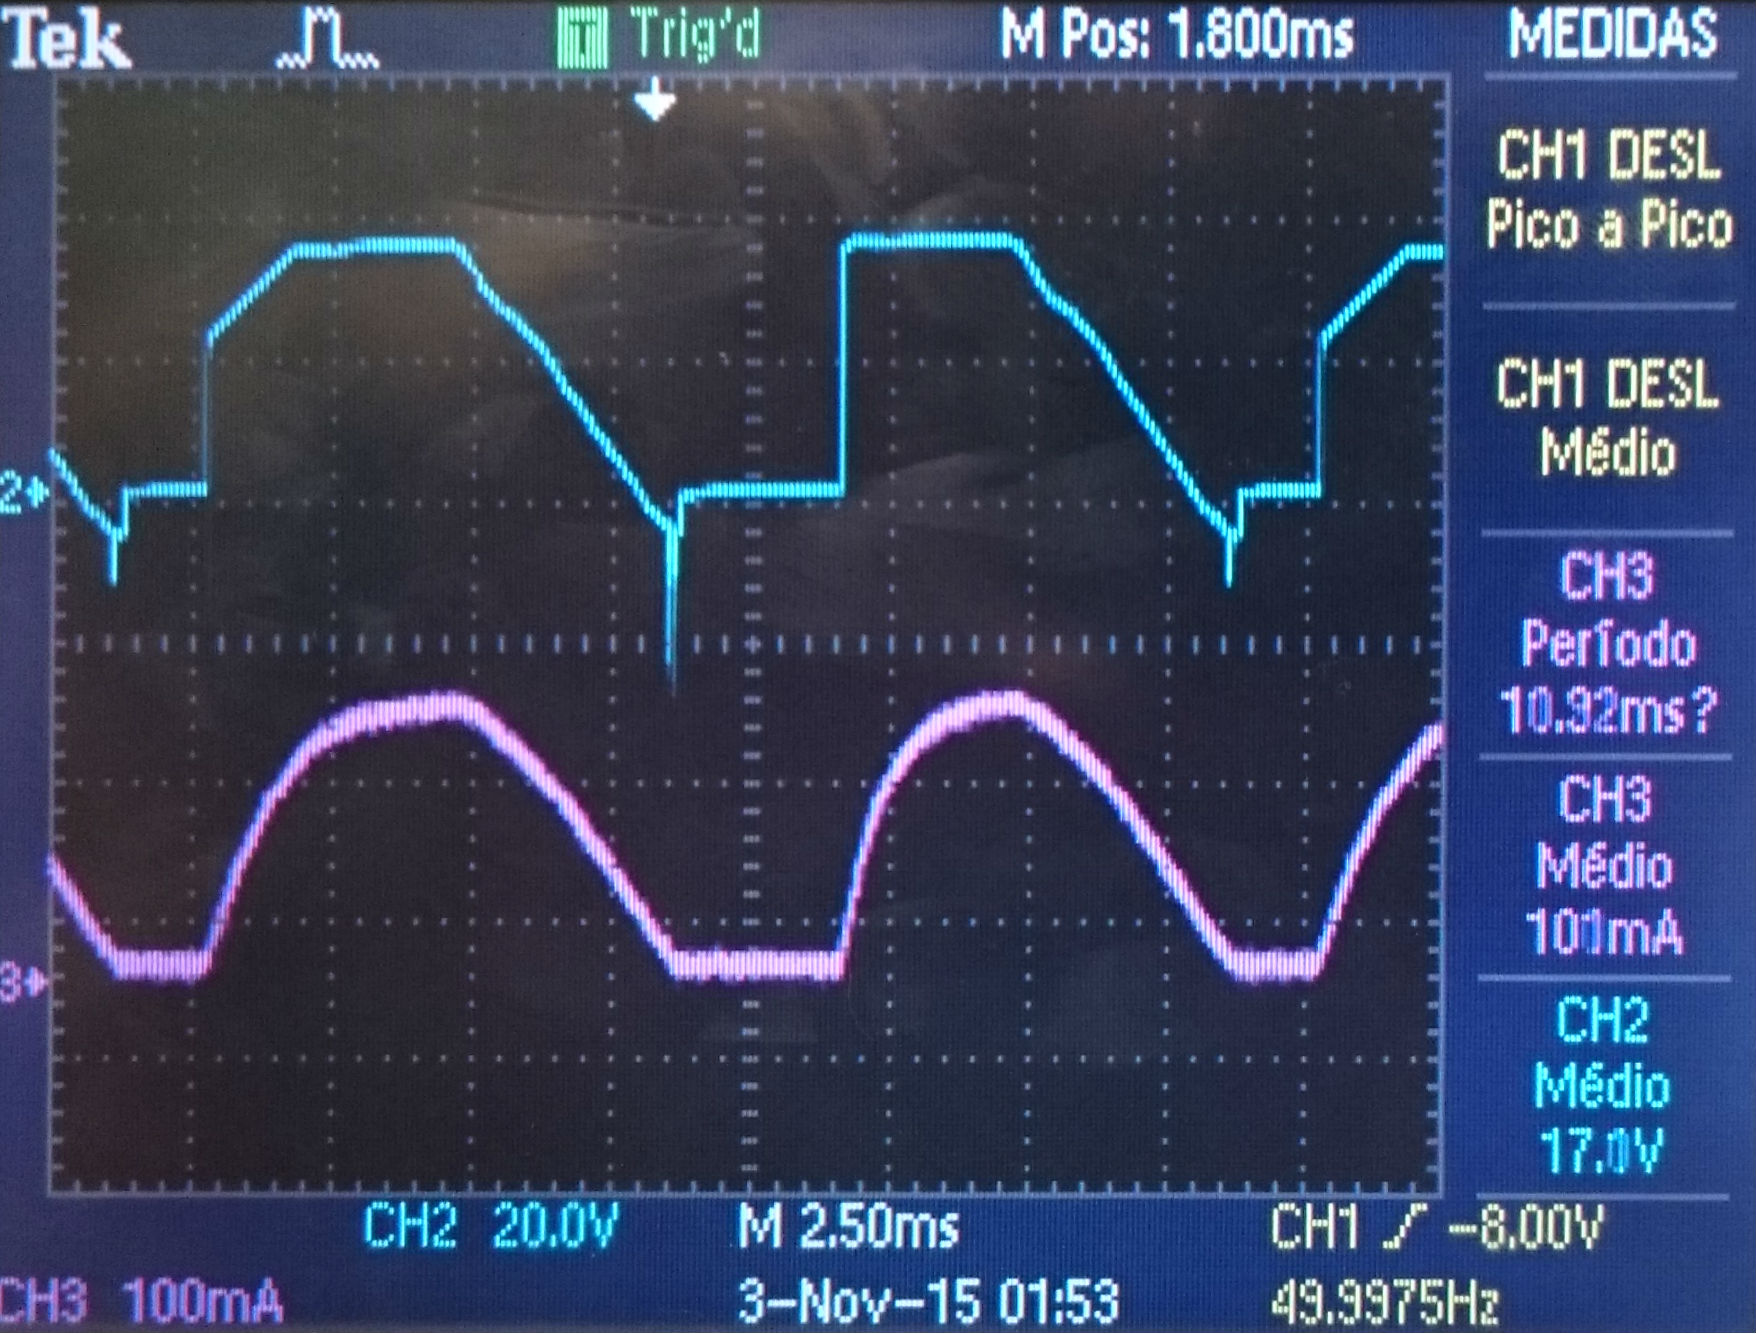
\includegraphics[keepaspectratio=true, scale=0.15]{img/DSC_0184}
	\caption{Tensão (a azul) e corrente (a rosa) na carga.}
	\label{fig:tcentradalacuna}
	\vspace{-0.8em}
\end{figure}

Quando a tensão se anula, ainda existe corrente. Assim, a condução do tirístor continua até que esta se anule, quando a tensão já está na arcada negativa.

A tensão média na bobina é necessariamente $0\,V$ (caso contrário, a corrente na bobina dispararia para infinito, queimando-se entretanto), pelo que a tensão média da resistência é igual à tensão média na carga.

\paragraph{Formas de onda da tensão e corrente no tiristor} \mbox{}\

Em cada braço do rectificador vai passar a corrente correspondente a uma das arcadas.

\begin{figure}[H]
	\centering
	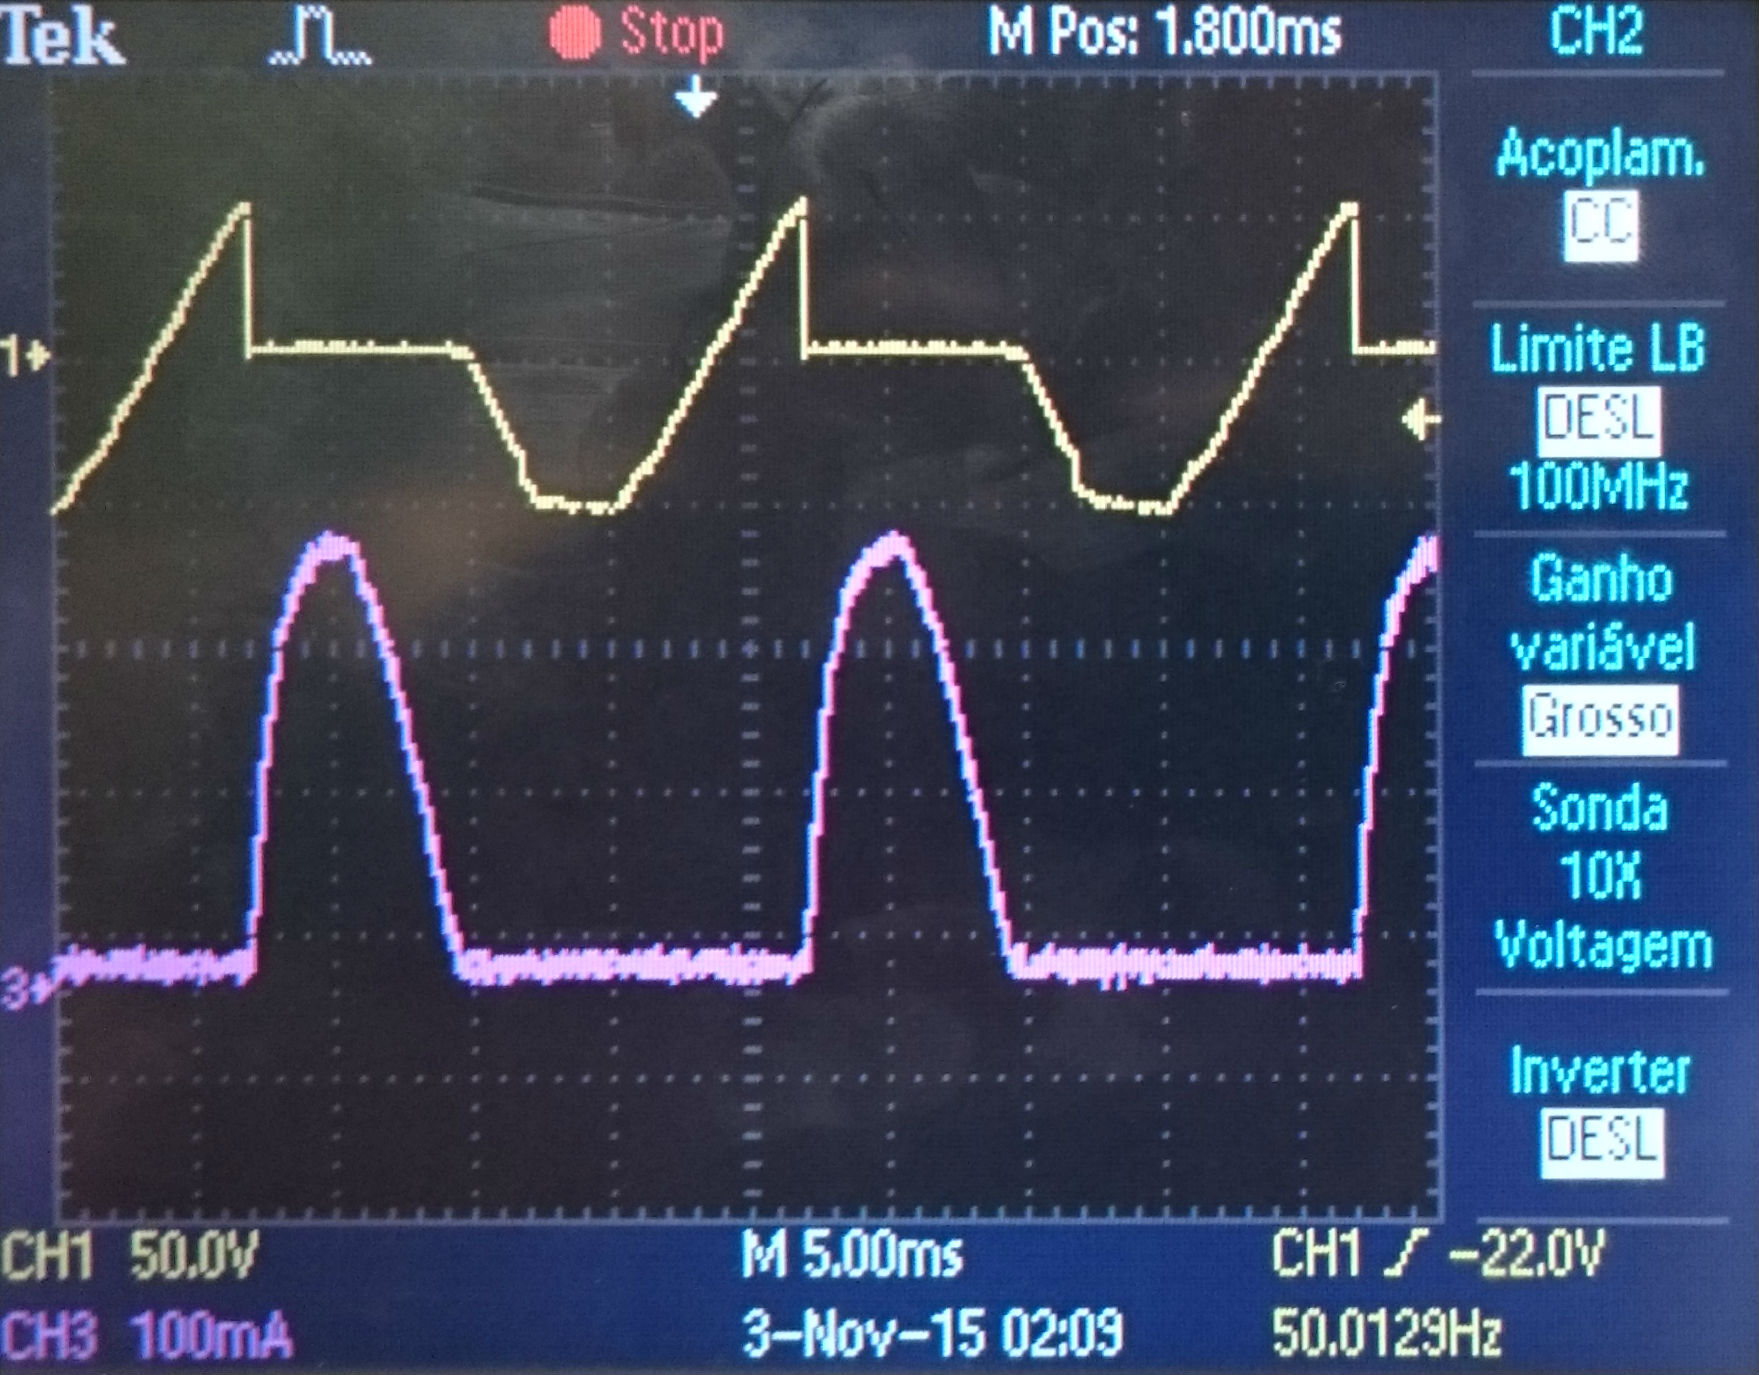
\includegraphics[keepaspectratio=true, scale=0.15]{img/DSC_0185}
	\caption{Tensão (a amarelo) e corrente (a rosa) no tiristor.}
	\label{fig:tctiristorlacuna}
	\vspace{-0.8em}
\end{figure}

%\paragraph{Formas de onda da tensão e corrente para funcionamento não lacunar} \mbox{}\
% Não temos isto. Não sei se a prof repara se não pusermos.

\paragraph{Característica de comando do conversor} \mbox{}\

As previsões teóricas foram feitas com recurso às Equações \ref{eq:teo1} a \ref{eq:teo4}.

\begin{equation}
\label{eq:teo1}
\Phi = \arctan{(\frac{\omega L}{R})}
\end{equation}

\begin{equation}
\label{eq:teo2}
0 = \sin{(\Phi - \alpha)}\,e^{-\frac{R}{L}\frac{\gamma}{\omega}}+\sin{(\alpha + \gamma - \phi)}
\end{equation}

\begin{equation}
\label{eq:teo3}
\overline{v_O} = \frac{1}{\pi} \int_\alpha^{\alpha+\gamma} \sqrt{2}V\,\sin{(\omega\,t)} \mathrm{d}\omega t
\end{equation}

\begin{equation}
\label{eq:teo4}
\overline{v_O} = \frac{\sqrt{2}V}{\pi} \left(-\cos{(\alpha + \gamma)}+\cos{(\alpha)}\right)
\end{equation}

Uma vez calculados os valores de $\gamma$ através da \autoref{eq:teo2}, foram calculados os valores médios da tensão graças à \autoref{eq:teo3}, para todos os valores de $\alpha$ excepto $\alpha = 0^\circ$.

Para $\alpha = 0^\circ$, como $\alpha < \Phi$, o circuito funciona em regime não lacunar, pelo que o valor teórico foi calculado com recurso à \autoref{eq:comandado_tensao}.

\begin{table}[H]
\centering
\begin{tabular}{c c c c c c c}
\hfil & Ângulo de Disparo $[^\circ]$ & \hfil & $V_O\;[V]$ (teórico) & \hfil & $V_O\;[V]$ (experimental) & \hfil \\
\hline
			&$0$&	&$31.5$&		&$31.9$&\\
\rowcolor{SkyBlue}	&$30$&	&$29.1$&		&$26.5$&\\
			&$60$&	&$23.4$&		&$19$&\\
\rowcolor{SkyBlue}	&$90$&	&$15.5$&		&$11.2$&\\
			&$120$&	&$7.6$&			&$4.7$&\\
\rowcolor{SkyBlue}	&$150$&	&$1.87$&		&$0.6$&\\
\hline
\end{tabular}
\caption{Valor médio da tensão de saída em função do ângulo de disparo ($V_i = 35 V$)}
\label{tab:akpklac}
\end{table}

\begin{figure}[H]
	\centering
	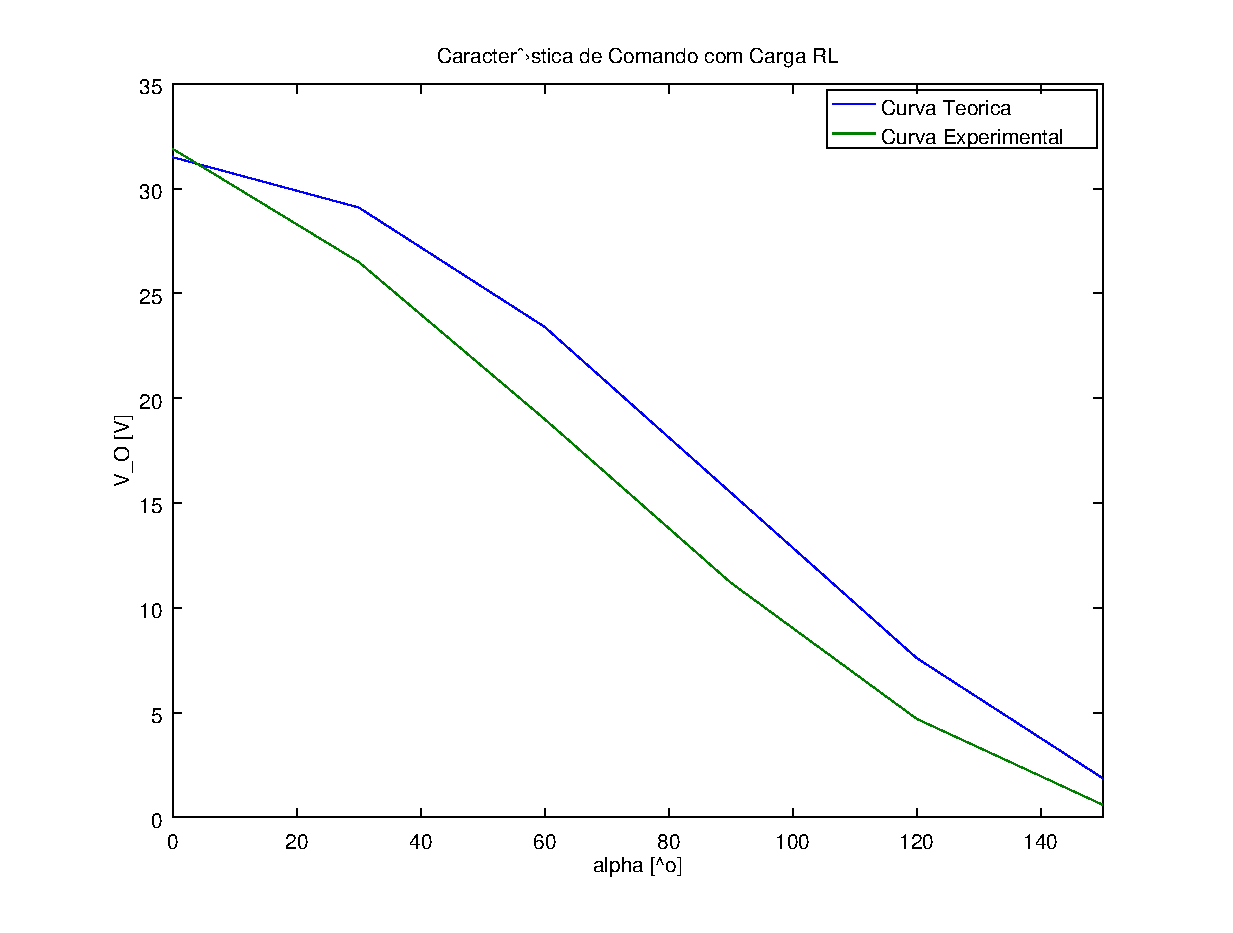
\includegraphics[keepaspectratio=true, width=0.8\textwidth]{img/comando2}
	\caption{Características teórica e experimental}
	\label{fig:comando2}
	\vspace{-0.8em}
\end{figure}

Na \autoref{fig:comando2} pode observar-se a previsão teórica da característica face aos valores obtidos. A diferença pode dever-se a diversos factores, como a dificuldade de colocação do reóstato no valor pretendido, bem como diversas outras imperfeições nos dispositivos.

Uma vez mais, o sinal de entrada não é uma sinusóide perfeita (longe disso), pelo que esse factor também interfere com a característica.

\subsection{Rectificador de onda completa semi-comandado}

\begin{figure}[H]
	\centering
	%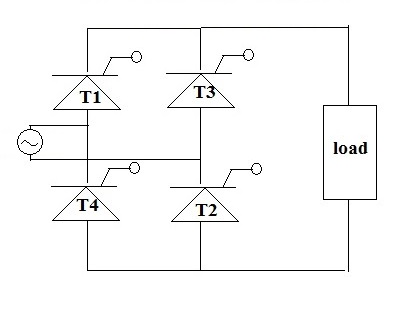
\includegraphics[keepaspectratio=true, scale=0.8]{img/circuito}
	\begin{tikzpicture}[scale=0.7, transform shape]
	\draw
		(0,0) node[] (origin) {} to[sV] ++(0,2) node[] (source) {}
		(origin) to[short,-*] ++ (5,0) to[short] ++ (0,2) to[Ty,l_=$T3$,-*] ++ (0,2) to[short] ++ (2,0) to[generic,l=Carga] ++ (0,-6) to[short] ++ (-2,0) node[] (bottomty) {} to[short] ++(-2,0) to[D, l_=$D4$] ++ (0,2) to[short,-*] ++ (0,2) node[] (topty) {} to[short] (source)
		(bottomty) to[D,l_=$D2$,*-*] ++ (0,2)
		(topty) to[Ty,l_=$T1$] ++(0,2) to[short] ++ (2,0)
		;
	\end{tikzpicture}
	\caption{Esquema do rectificador de onda completa monofásico semi-comandado}
	\label{fig:circuit_2}
	\vspace{-0.8em}
\end{figure}

De maneira a observar o funcionamento do Rectificador semi-comandado, os tirístores $T2$ e $T4$, isto é, os correspondentes ao troço inferior de cada braço do rectificador, foram substituídos por díodos.

\subsubsection{Carga indutiva RL}

\paragraph{Formas de onda da tensão e corrente na entrada} \mbox{}\

\begin{figure}[H]
	\centering
	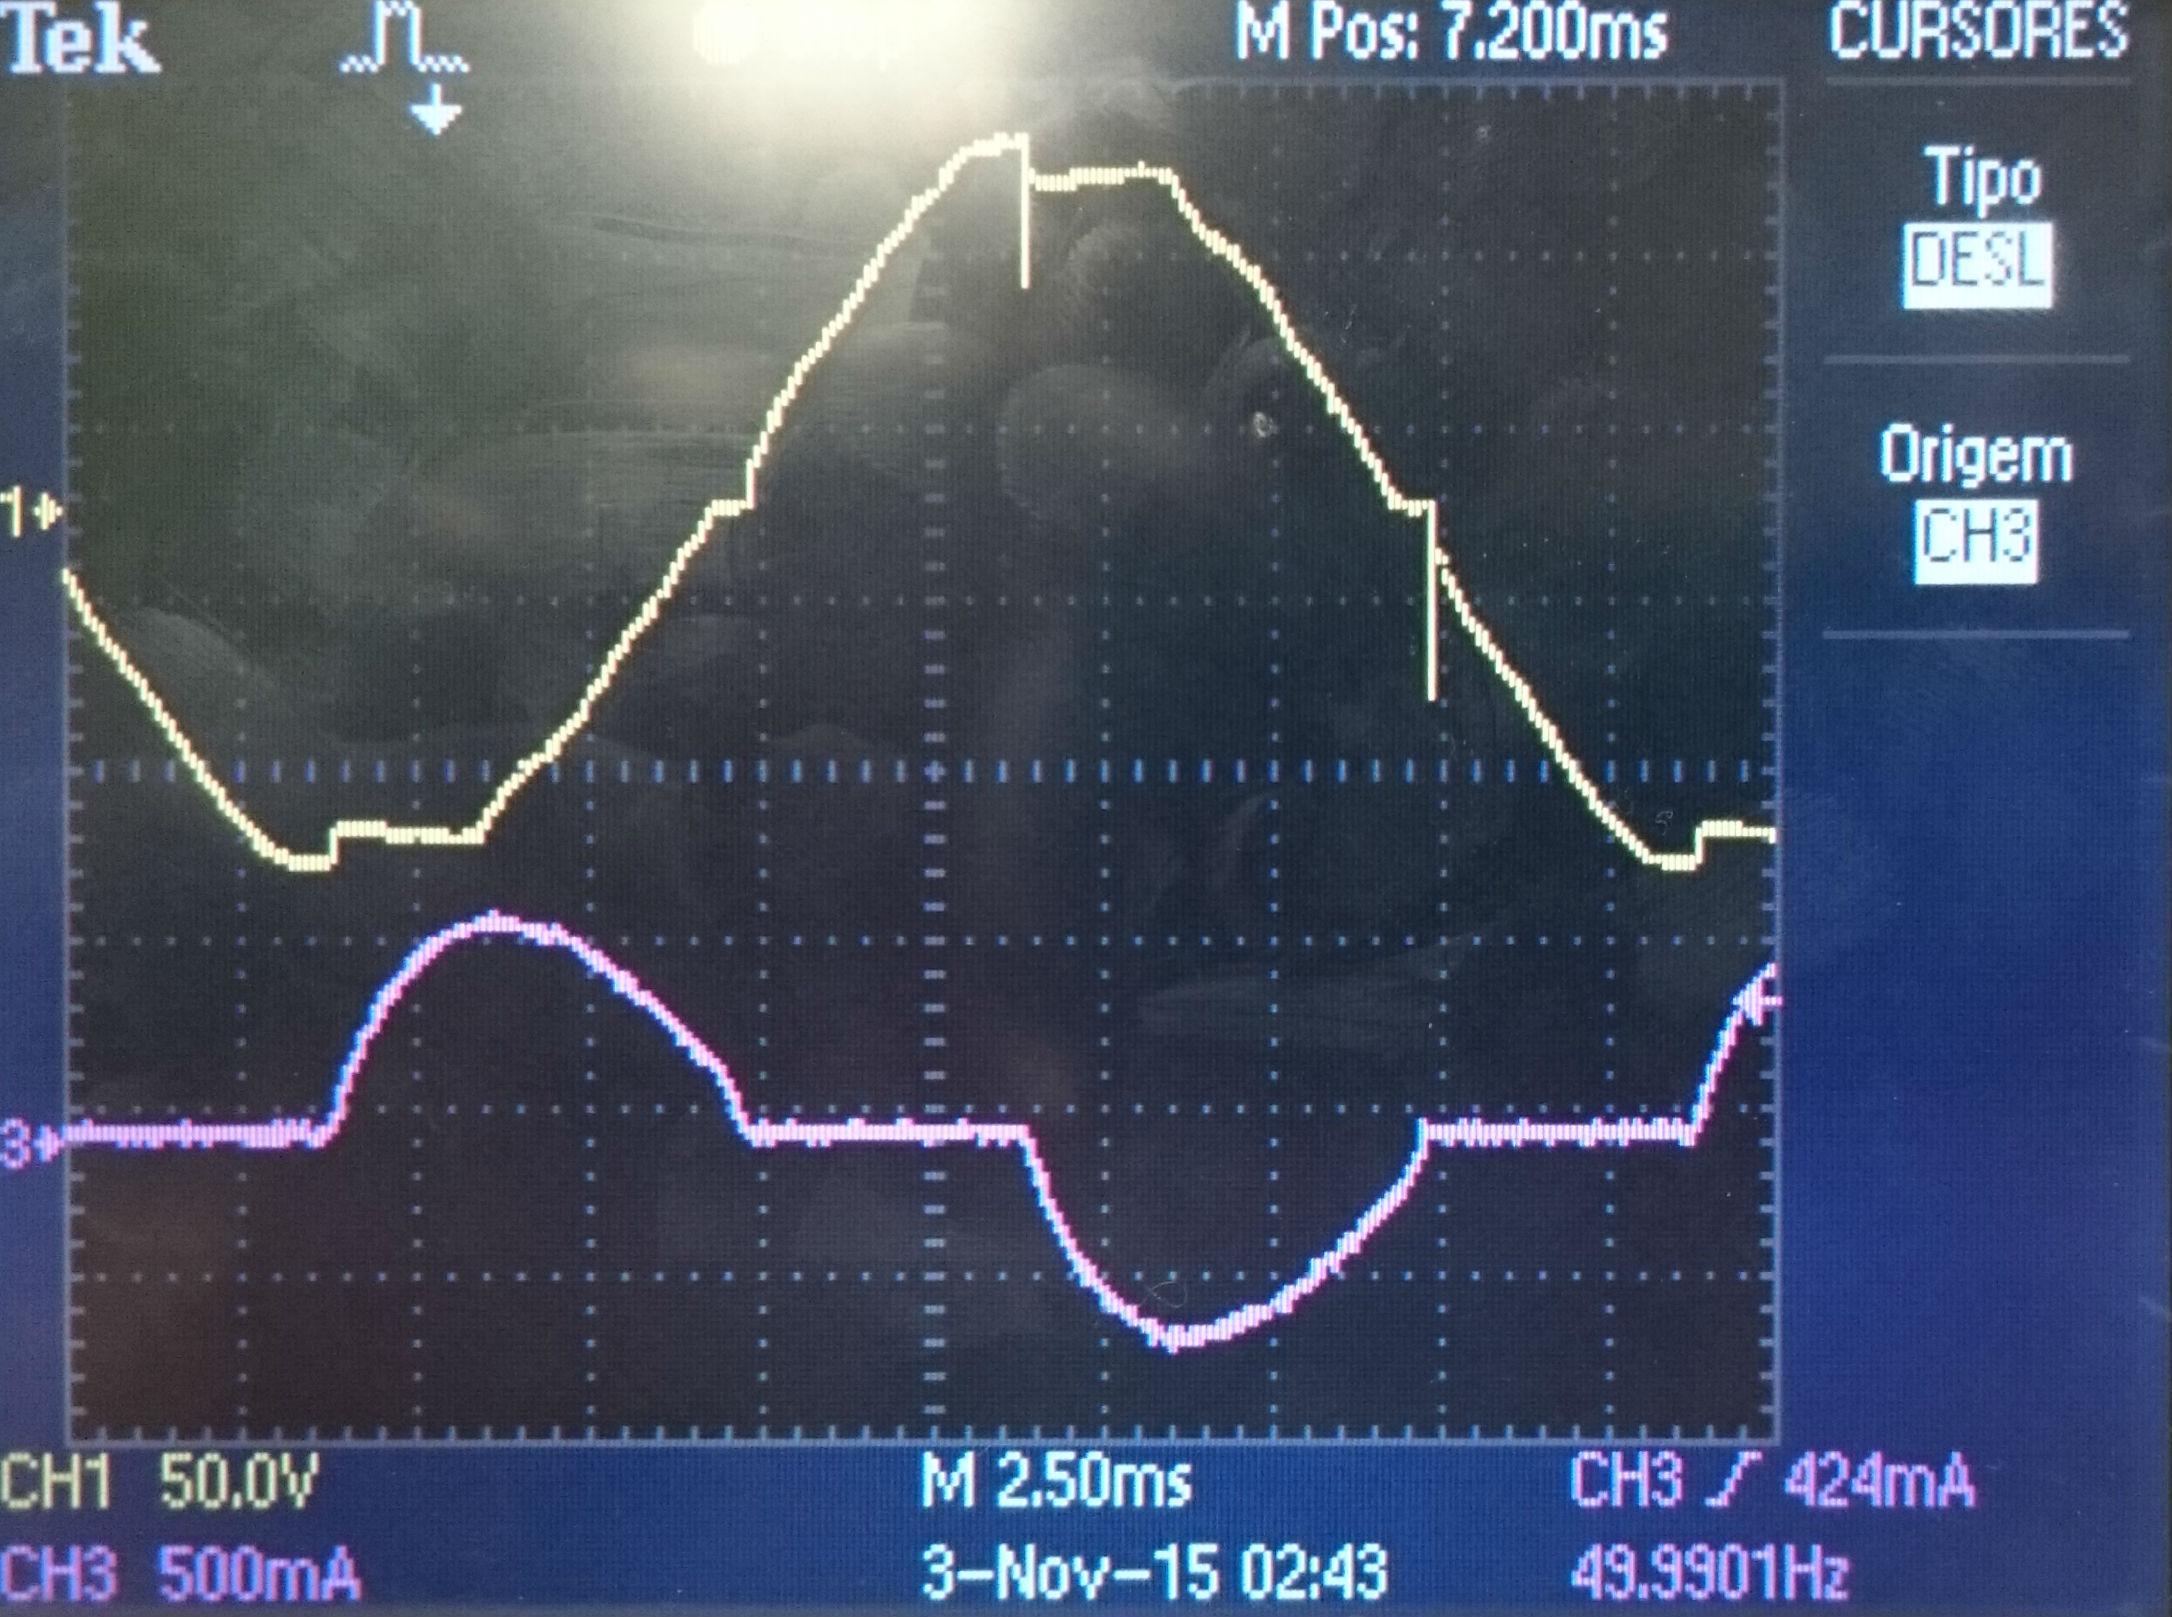
\includegraphics[keepaspectratio=true, scale=0.12]{img/DSC_0190}
	\caption{Tensão (a amarelo) e corrente (a rosa) na entrada.}
	\label{fig:tcentradasemi}
	\vspace{-0.8em}
\end{figure}

Na entrada do circuito, é possível observar pequenos picos na tensão sempre que um dispositivo (tirístor ou díodo) passam da condução ao corte, e vice versa.

\paragraph{Formas de onda da tensão e corrente na carga} \mbox{}\

\begin{figure}[H]
	\centering
	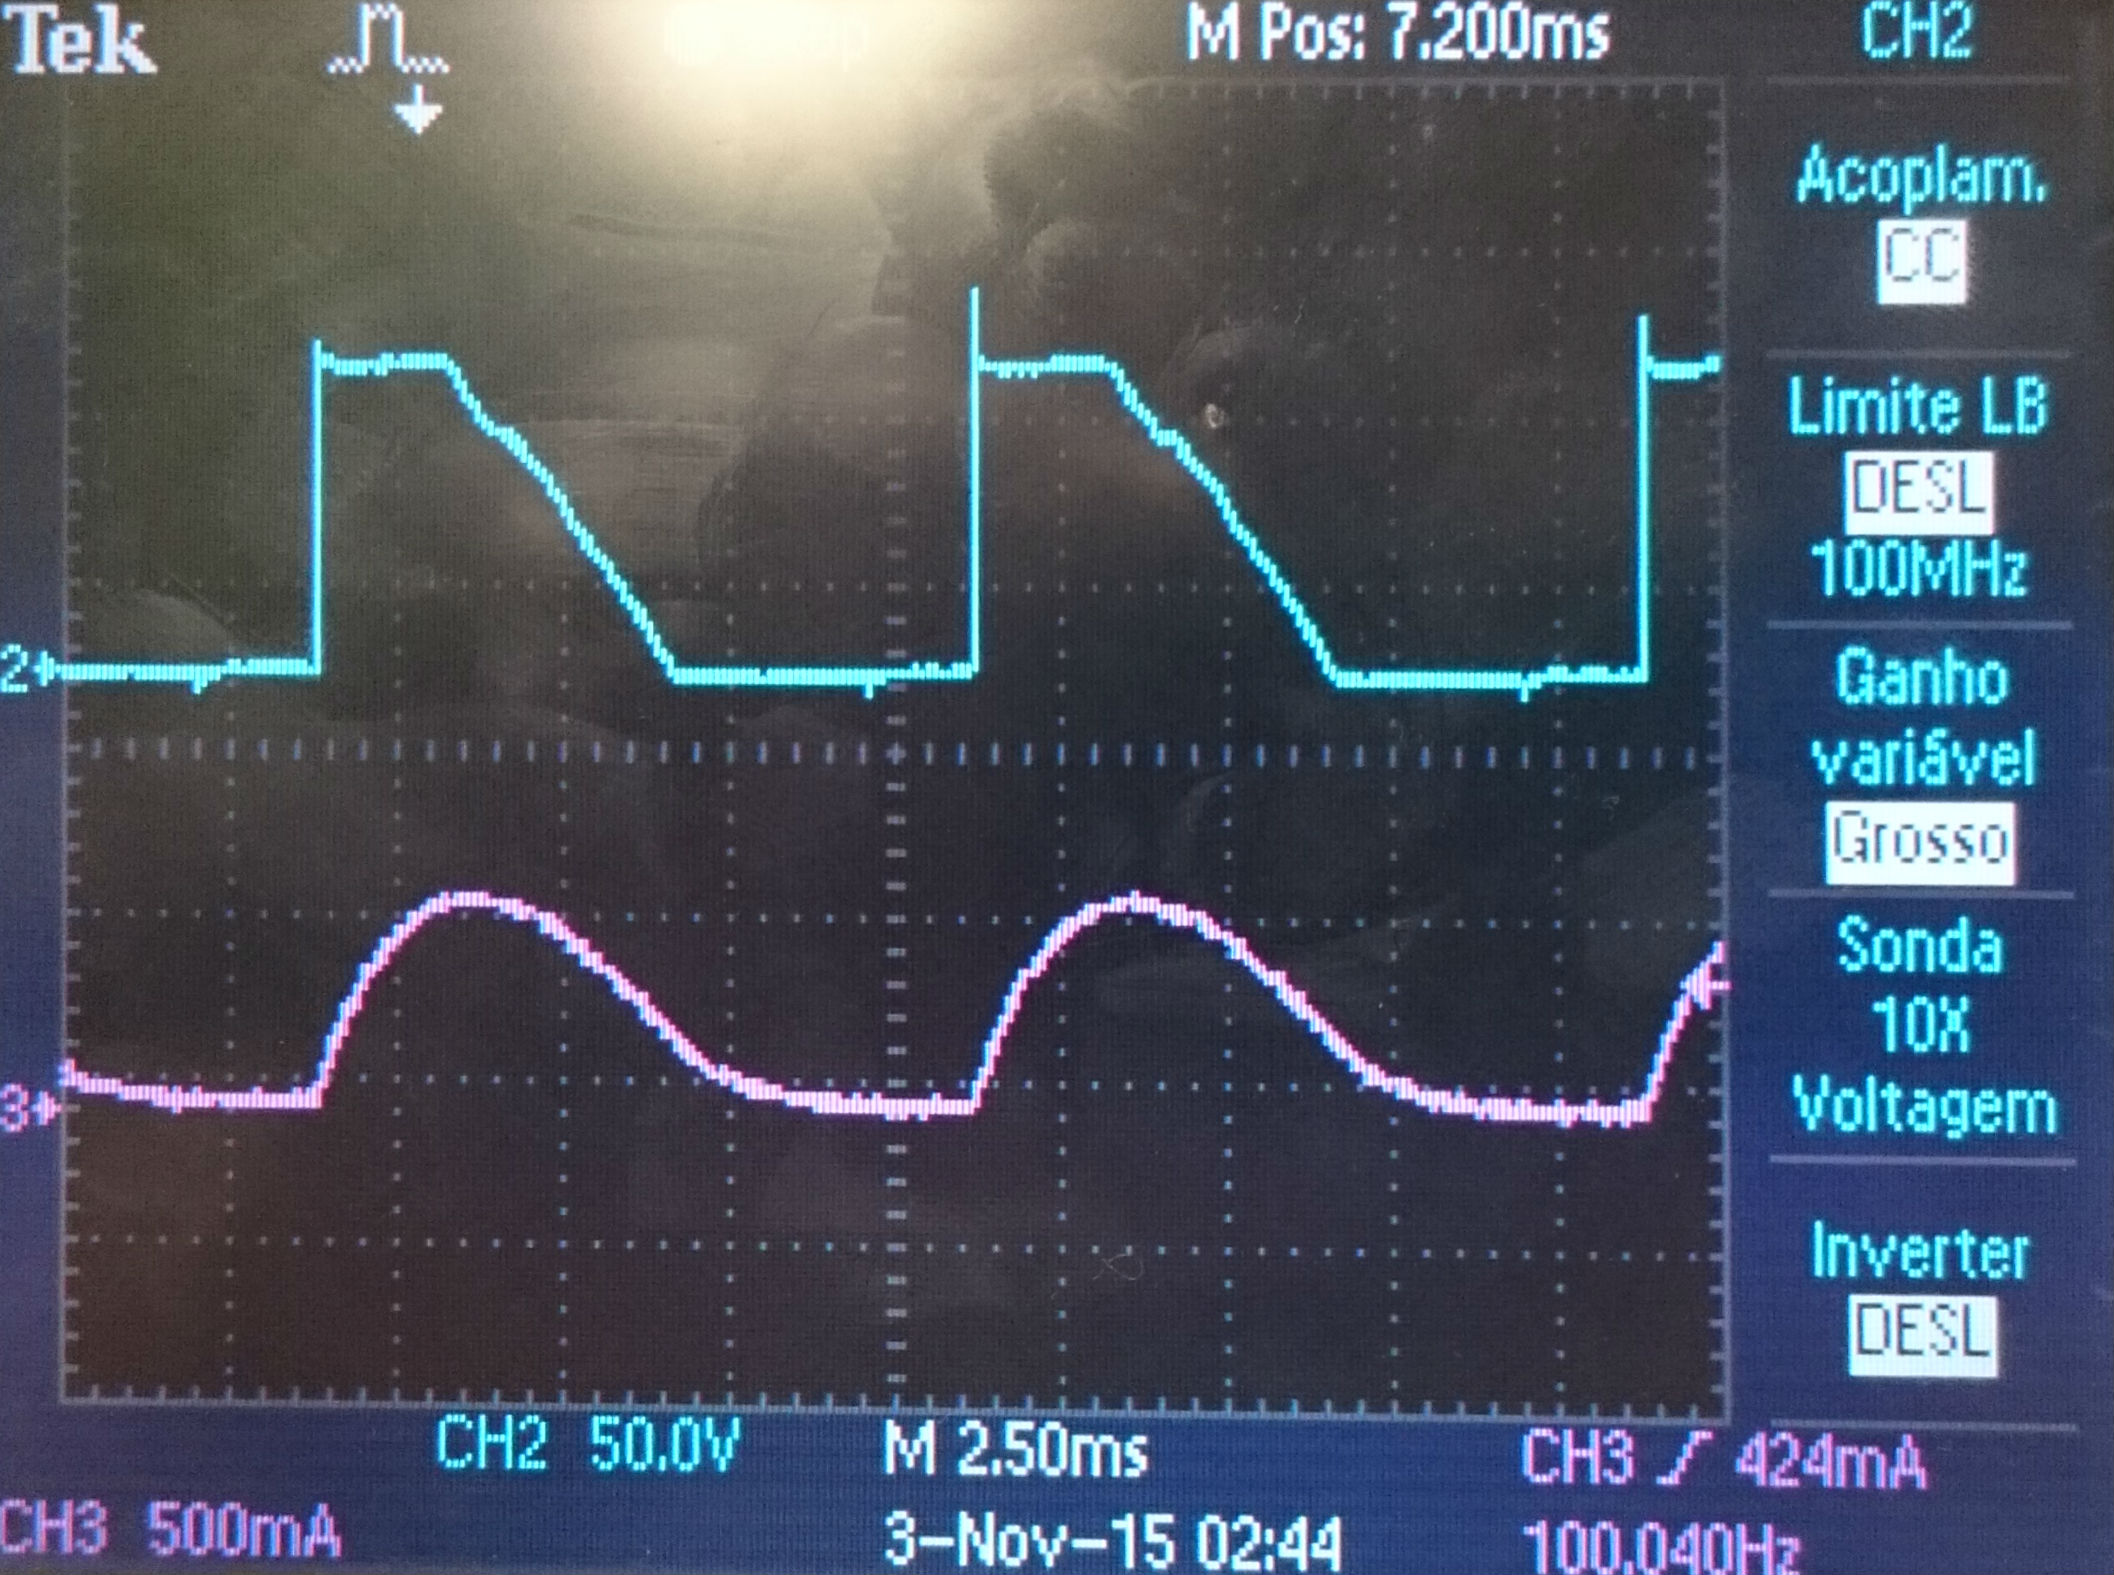
\includegraphics[keepaspectratio=true, scale=0.13]{img/DSC_0191}
	\caption{Tensão (a azul) e corrente (a rosa) na carga.}
	\label{fig:tccargasemi}
	\vspace{-0.8em}
\end{figure}

Na carga verifica-se que a tensão é sempre positiva, ao contrário da situação anterior. Uma vez que continua a haver a mesma inércia da corrente (causada pela bobina), a justificação pela qual a tensão deixa de tomar valores negativos só se pode dever à substituição dos dois tirístores por díodos.

Após constatar esse facto, é fácil perceber que os tirístores necessitam impulso de gate para conduzir, que os díodos, evidentemente, não precisam.

Assim, quando a tensão de alimentação passa à arcada negativa, a continuidade da corrente da carga é assegurada pelos díodos (na situação anterior, como os tirístores não tinham impulso de gate nesse instante, o mesmo não se verificava).

\paragraph{Formas de onda da tensão e corrente nos díodos} \mbox{}\

\begin{figure}[H]
	\centering
	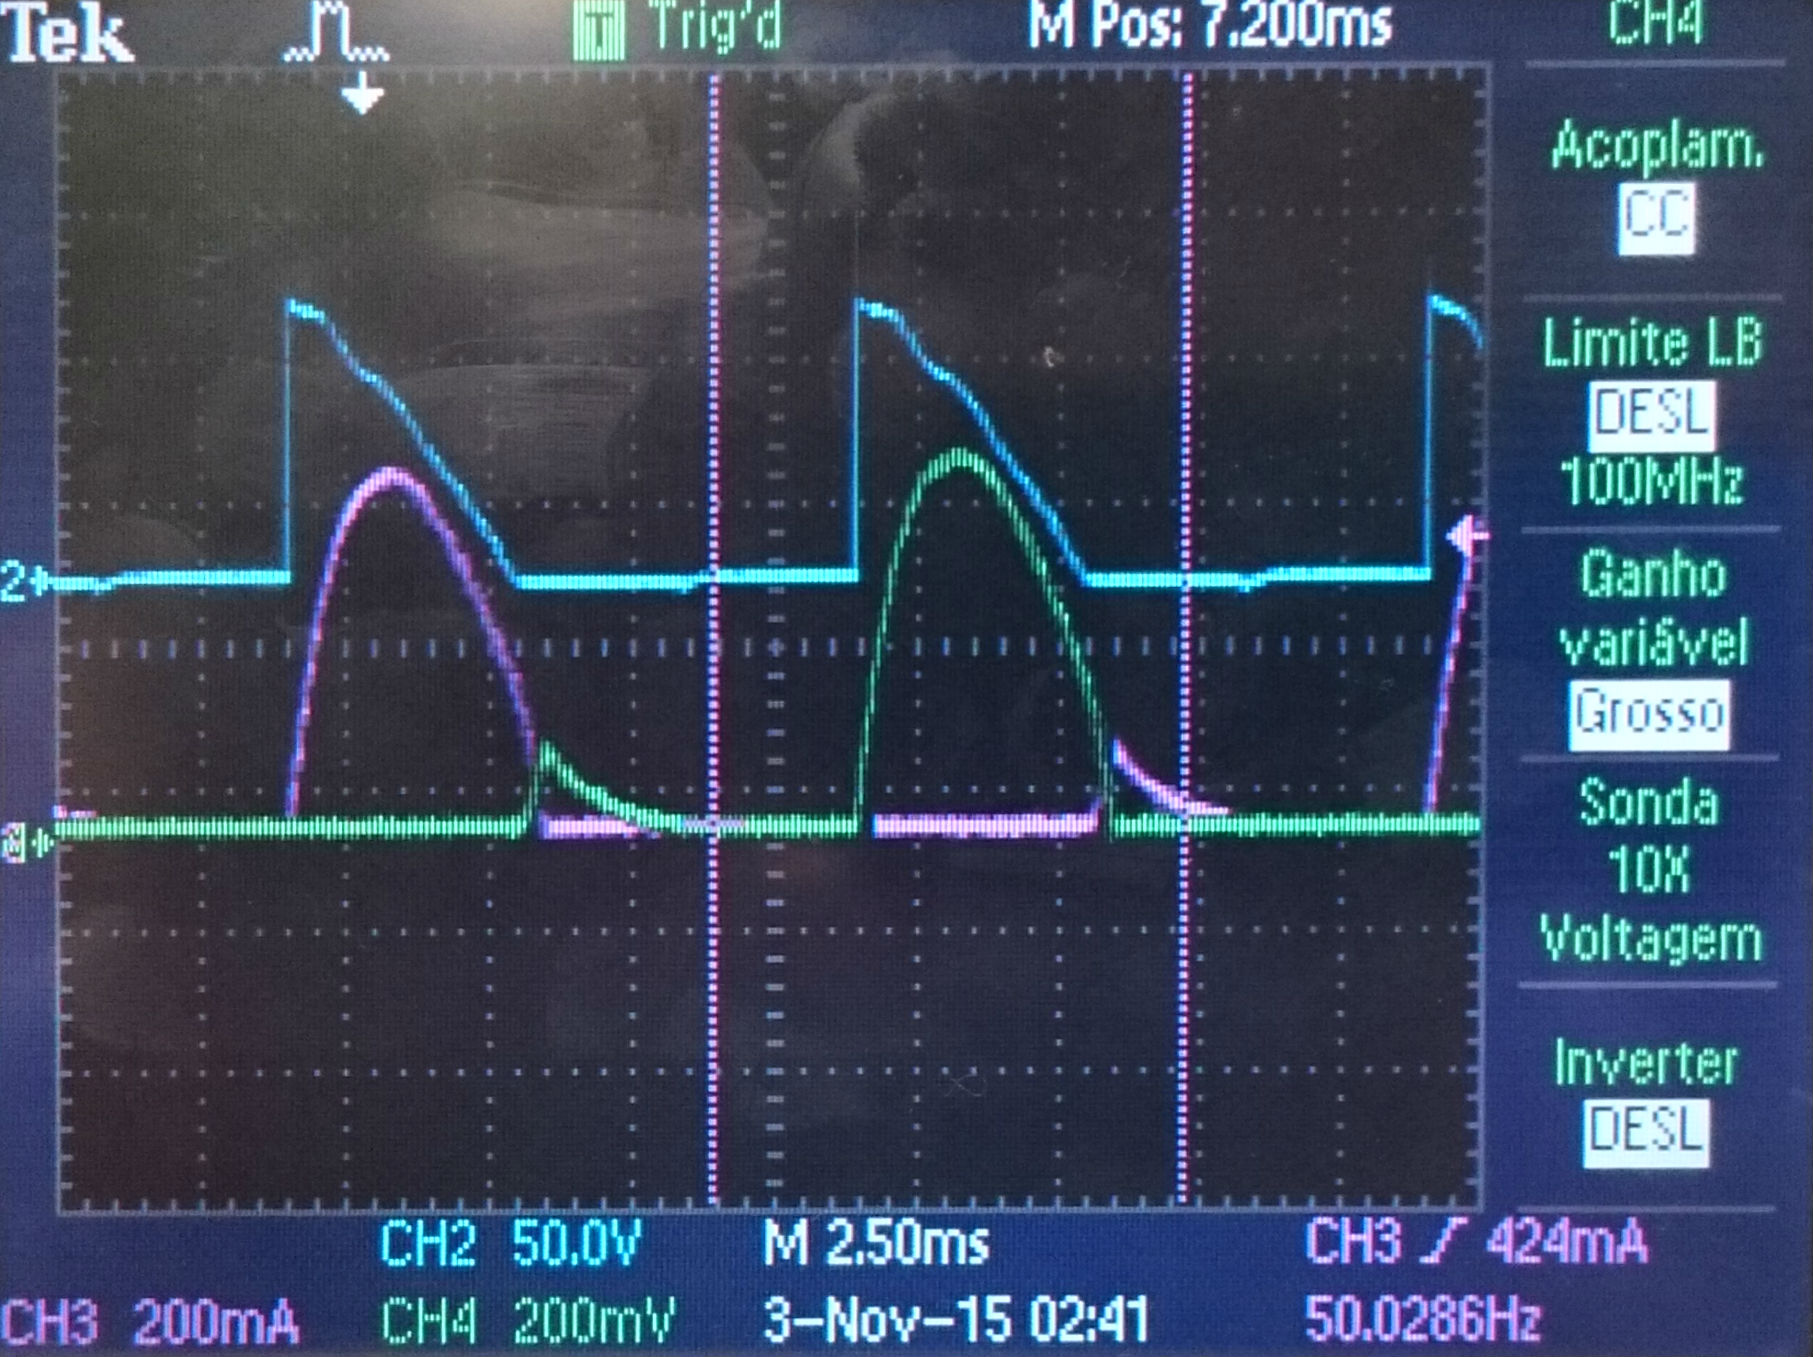
\includegraphics[keepaspectratio=true, scale=0.12]{img/DSC_0189}
	\caption{Tensão de saída (a azul), corrente em um dos díodos (a rosa), e corrente no díodo complementar (a verde)}
	\label{fig:rsemidiodos}
	\vspace{-0.8em}
\end{figure}

É possível observar a continuidade da corrente garantida pelos díodos complementares entre si, sendo que a soma das correntes dos dois díodos corresponde à corrente da carga.

\paragraph{Característica de comando do conversor} \mbox{}\


De maneira a calcular o valor médio da tensão na carga, foi utilizada uma expressão semelhante à \autoref{eq:teo3} da questão anterior, mas uma vez que independentemente do ângulo de condução $\gamma$, a tensão é cortada para $\omega t = \pi$, o limite superior de integração da tensão é $\pi$.

A expressão resultante é portanto idêntica à da tensão média para o rectificador de onda completa totalmente controlado (\autoref{eq:comandado_tensao}).

\begin{table}[H]
\centering
\begin{tabular}{c c c c c c c}
\hfil & Ângulo de Disparo $[^\circ]$ & \hfil & $V_O\;[V]$ (teórico) & \hfil & $V_O\;[V]$ (experimental) & \hfil \\
\hline
			&$0$&	&$72.03$&		&$72.7$&\\
\rowcolor{SkyBlue}	&$30$&	&$67.2$&		&$69.8$&\\
			&$60$&	&$54.02$&		&$53.2$&\\
\rowcolor{SkyBlue}	&$90$&	&$36.01$&		&$39.5$&\\
			&$120$&	&$18.01$&		&$18.3$&\\
\rowcolor{SkyBlue}	&$150$&	&$4.82$&		&$4.73$&\\
\hline
\end{tabular}
\caption{Valor médio da tensão de saída em função do ângulo de disparo ($V_i = 80 V$)}
\label{tab:akpksemi}
\end{table}


\begin{figure}[H]
	\centering
	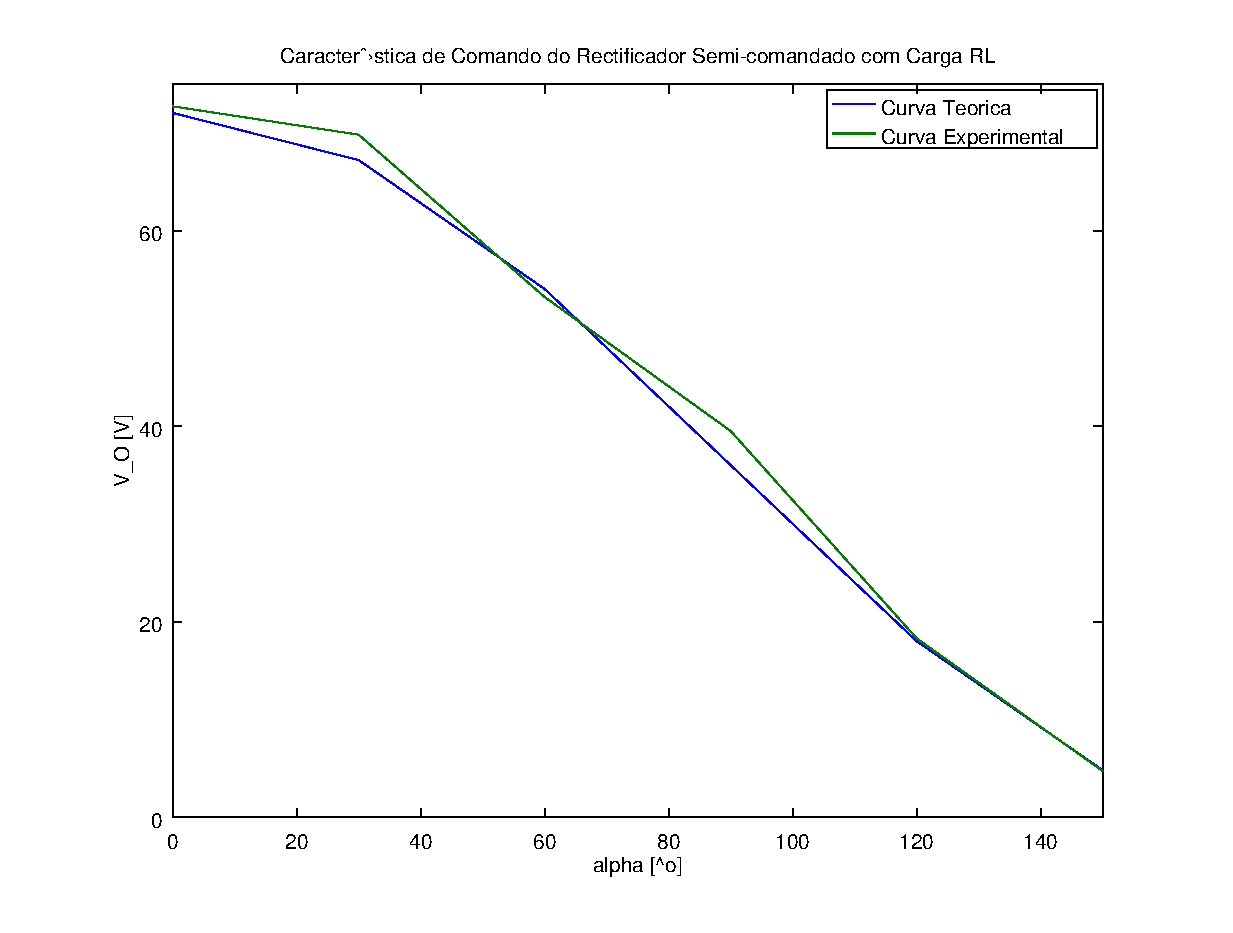
\includegraphics[keepaspectratio=true, width=0.8\textwidth]{img/comando3}
	\caption{Características teórica e experimental}
	\label{fig:comando3}
	\vspace{-0.8em}
\end{figure}

Na \autoref{fig:comando3} verifica-se uma melhor correspondência entre a previsão teórica e os resultados experimentais.

\paragraph{Conclusões} \mbox{}\

A corrente na carga nunca é negativa, uma vez que isso exigiria que pelo menos um dos dois díodos (ou, no caso anterior, pelo menos um dos dois tirístores) conduzisse enquanto inversamente polarizados. Isso levaria à destruição do dispositivo.

%\todo{valor médio da tensão na carga para ângulo de diaspor deo 60º} Isso está feito na característica de comando

%\todo{dizer se é possivel utilizar este circuito para controlar a velocidade de um motor CC com travagem regenerativa}

Como tal, seria impossível controlar um motor com travagem regenerativa, uma vez que o processo de devolução de potência à fonte exigiria correntes negativas na carga.

%\todo{que tipo de filtro utilizaria para exigências de conteúdo harmónico. Pode ligar-se um condensador em paralelo na saída do rectificador? porque?}

Um filtro de saída teria de ser um filtro de 1ª ordem na forma de uma bobina em série com a carga. Ao colocar um condensador, o valor mínimo da tensão de saída deixaria de ser $0$, pelo que os tiristores deixariam de conduzir em todos os ângulos de disparo $0\leq \alpha \leq \pi$. Para além dessa diminuição da margem de controlo sobre o circuito, a potência entregue pelo rectificador à carga também se reduz, o que é indesejável.


\pagebreak
\section{Simulações}
\subsection{Circuitos de Potência usados}

Neste projeto foram utilizados três circuitos de potência: um rectificador de onda completa totalmente comandado, quer com carga resistiva, quer com carga \textit{RL}, e um rectificador de onda completa semi-comandado com carga \textit{RL}. 

\begin{figure}[h]
	\centering
	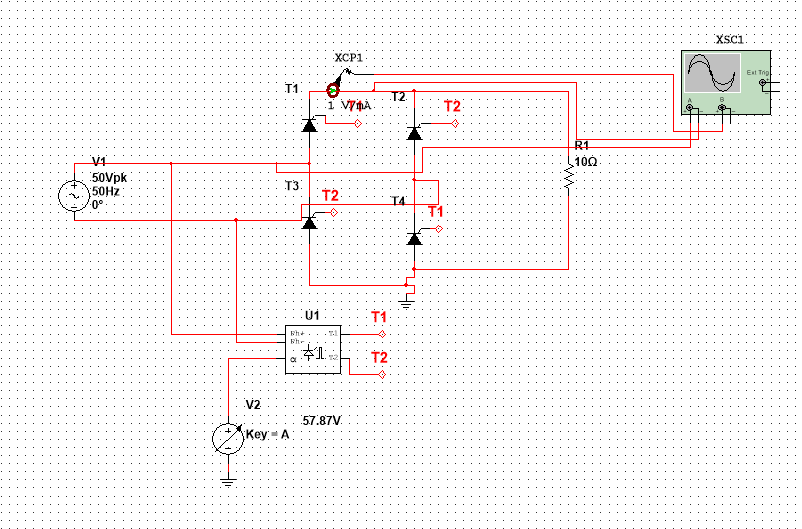
\includegraphics[keepaspectratio=true, scale=0.5]{img/circuito1}
	\caption{Rectificador de onda completa com comando total e carga resistiva, \textit{R}.}
	\label{fig:circuit_3}
	\vspace{-0.8em}
\end{figure}

\begin{figure}[h]
	\centering
	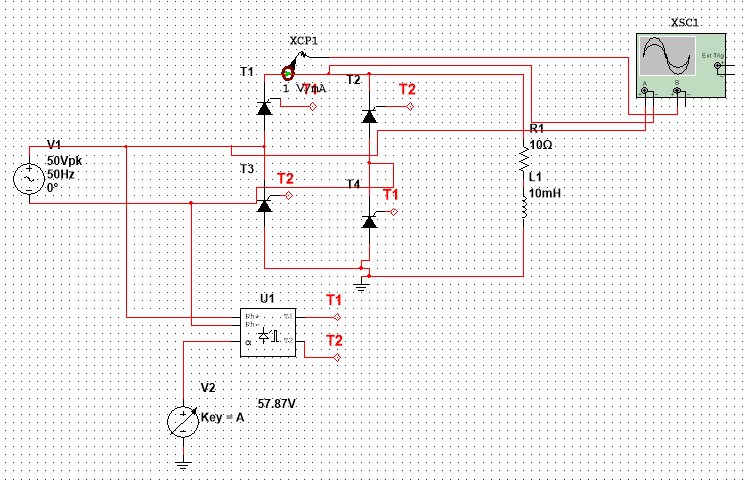
\includegraphics[keepaspectratio=true, scale=0.5]{img/circuito2}
	\caption{Rectificador de onda completa com comando total e carga \textit{RL}.}
	\label{fig:circuit_4}
	\vspace{-0.8em}
\end{figure}

\begin{figure}[h]
	\centering
	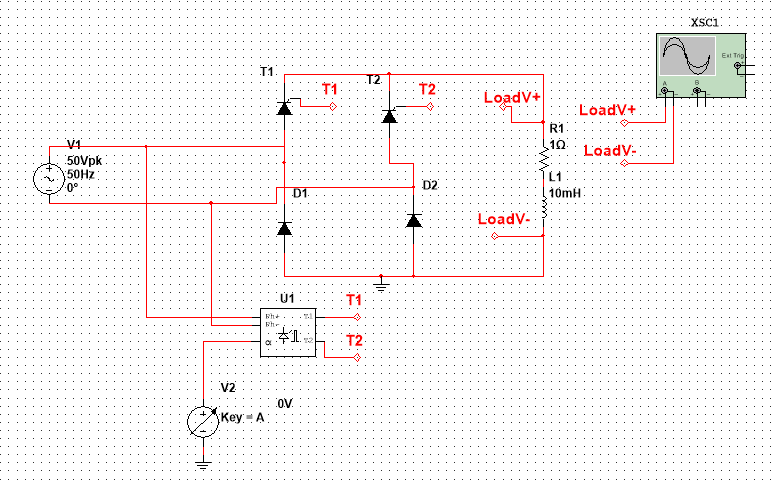
\includegraphics[keepaspectratio=true, scale=0.5]{img/circuito3}
	\caption{Rectificador onda completa semi-comandado e carga \textit{RL}.}
	\label{fig:circuit_5}
	\vspace{-0.8em}
\end{figure}
\pagebreak 

É importante referir que para a simulação do circuito de disparos se definiu que iria ser utilizado um \textit{drive} que impulsos com uma frequência  de $50Hz$. Pode-se controlar o ângulo de  disparo com uma fonte DC interactiva. Na \autoref{fig:circuit_6} está representado o sinal do gerador de impulsos com a tensão de entrada.
\vspace{17mm}

\begin{figure}[h]
	\centering
	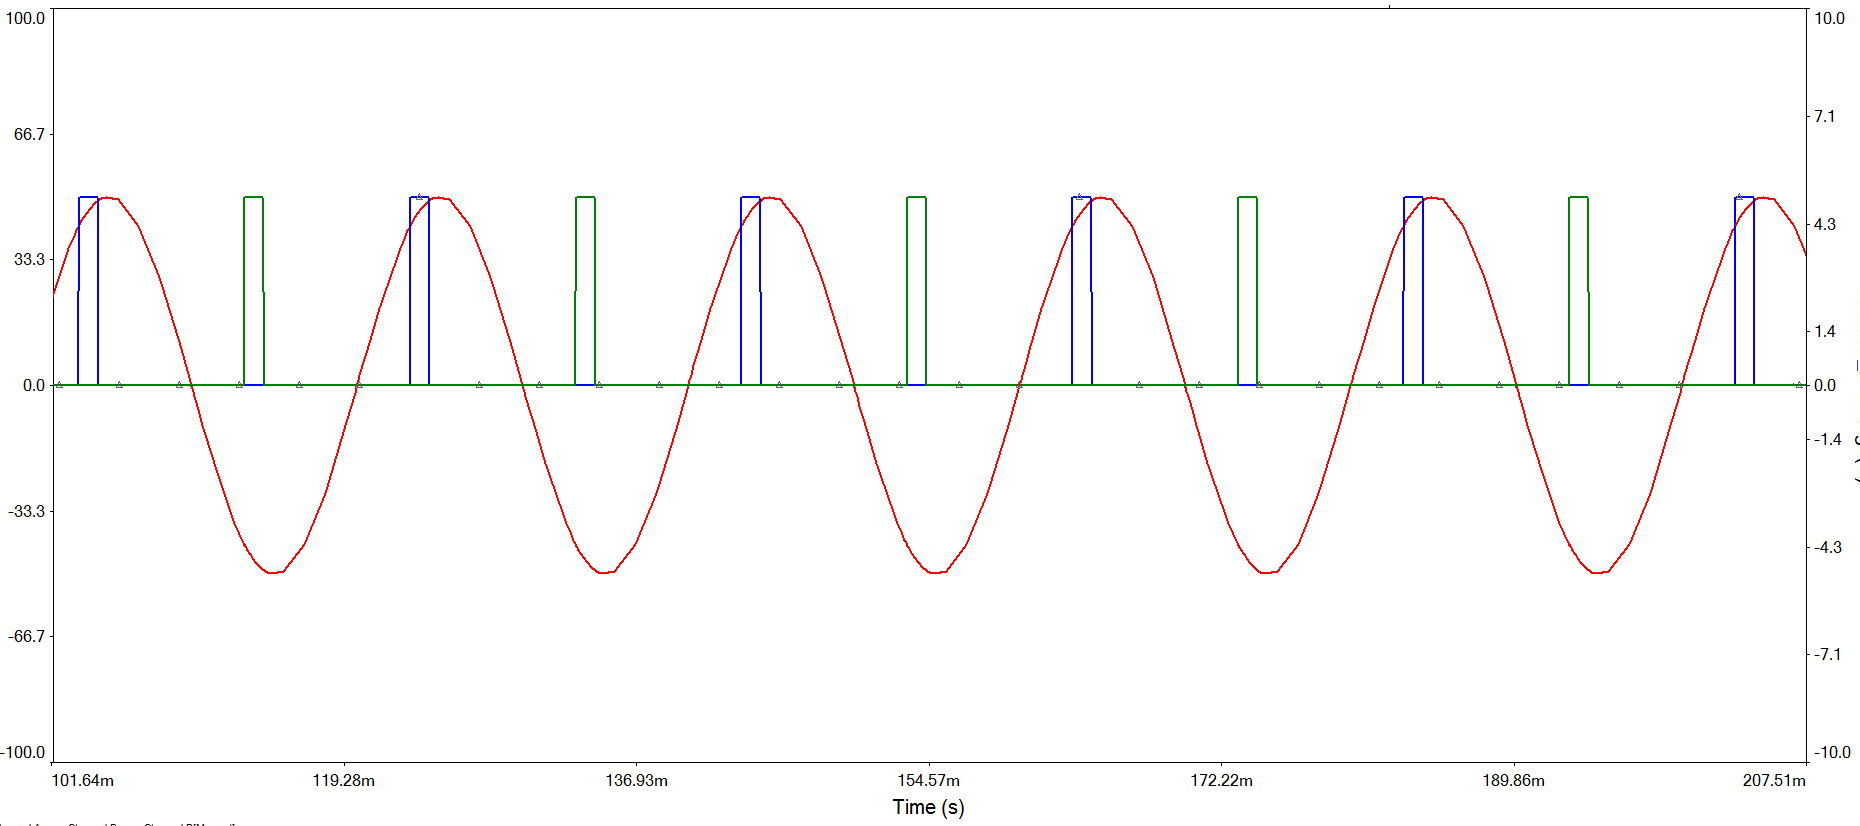
\includegraphics[keepaspectratio=true, scale=0.4]{img/circuito4}
	\caption{Tensão de entrada (sinal vermelho) e sinal da gate do tirístor (sinal azul), bem como o seu complementar (sinal a verde).}
	\label{fig:circuit_6}
	\vspace{-0.8em}
\end{figure}

\subsubsection{Rectificador de onda completa com comando total e carga resistiva, \textit{R}}

A \autoref{fig:circuit_7} tem representadas as formas de onda para a tensão e corrente de entrada.

\begin{figure}[h]
	\centering
	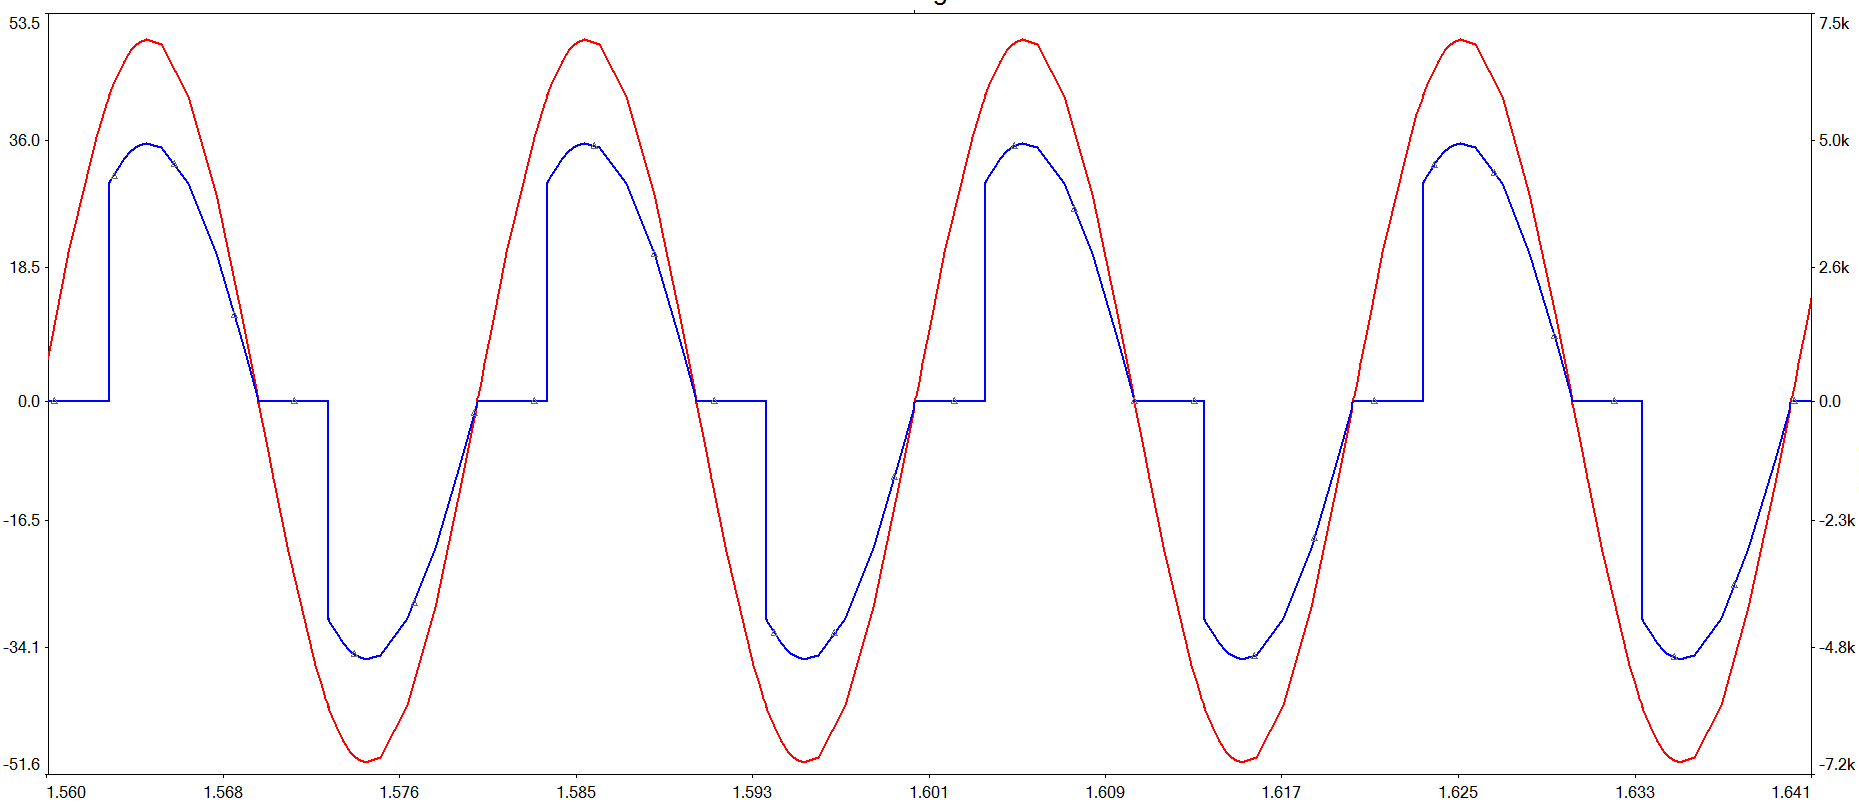
\includegraphics[keepaspectratio=true, scale=0.4]{img/circuito5}
	\caption{Tensão (sinal vermelho) e corrente (sinal azul) de entrada.}
	\label{fig:circuit_7}
	\vspace{-0.8em}
\end{figure}

\pagebreak
As formas de onda referentes à saída, isto é, à carga, podem ser visualizadas na \autoref{fig:circuit_8}.

\begin{figure}[h]
	\centering
	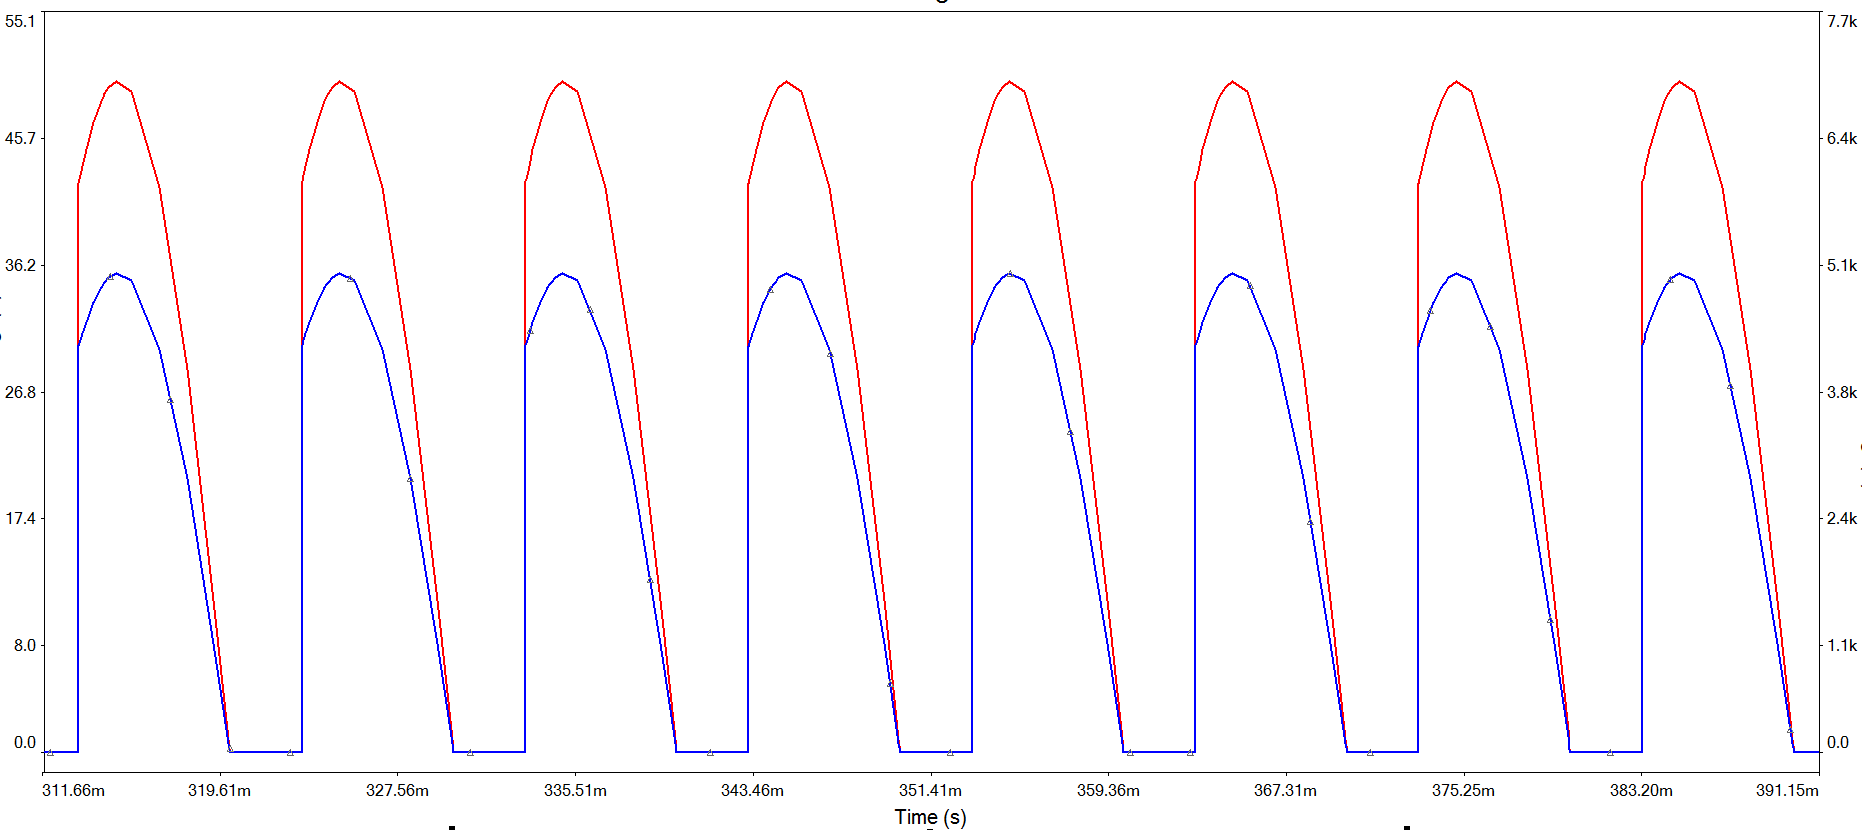
\includegraphics[keepaspectratio=true, scale=0.4]{img/circuito6}
	\caption{Tensão (sinal vermelho) e corrente (sinal azul) de saída.}
	\label{fig:circuit_8}
	\vspace{-0.8em}
\end{figure}

Já as formas de onda da tensão e da corrente de um dos tirístores podem ser visualizadas na \autoref{fig:circuit_9}

\begin{figure}[h]
	\centering
	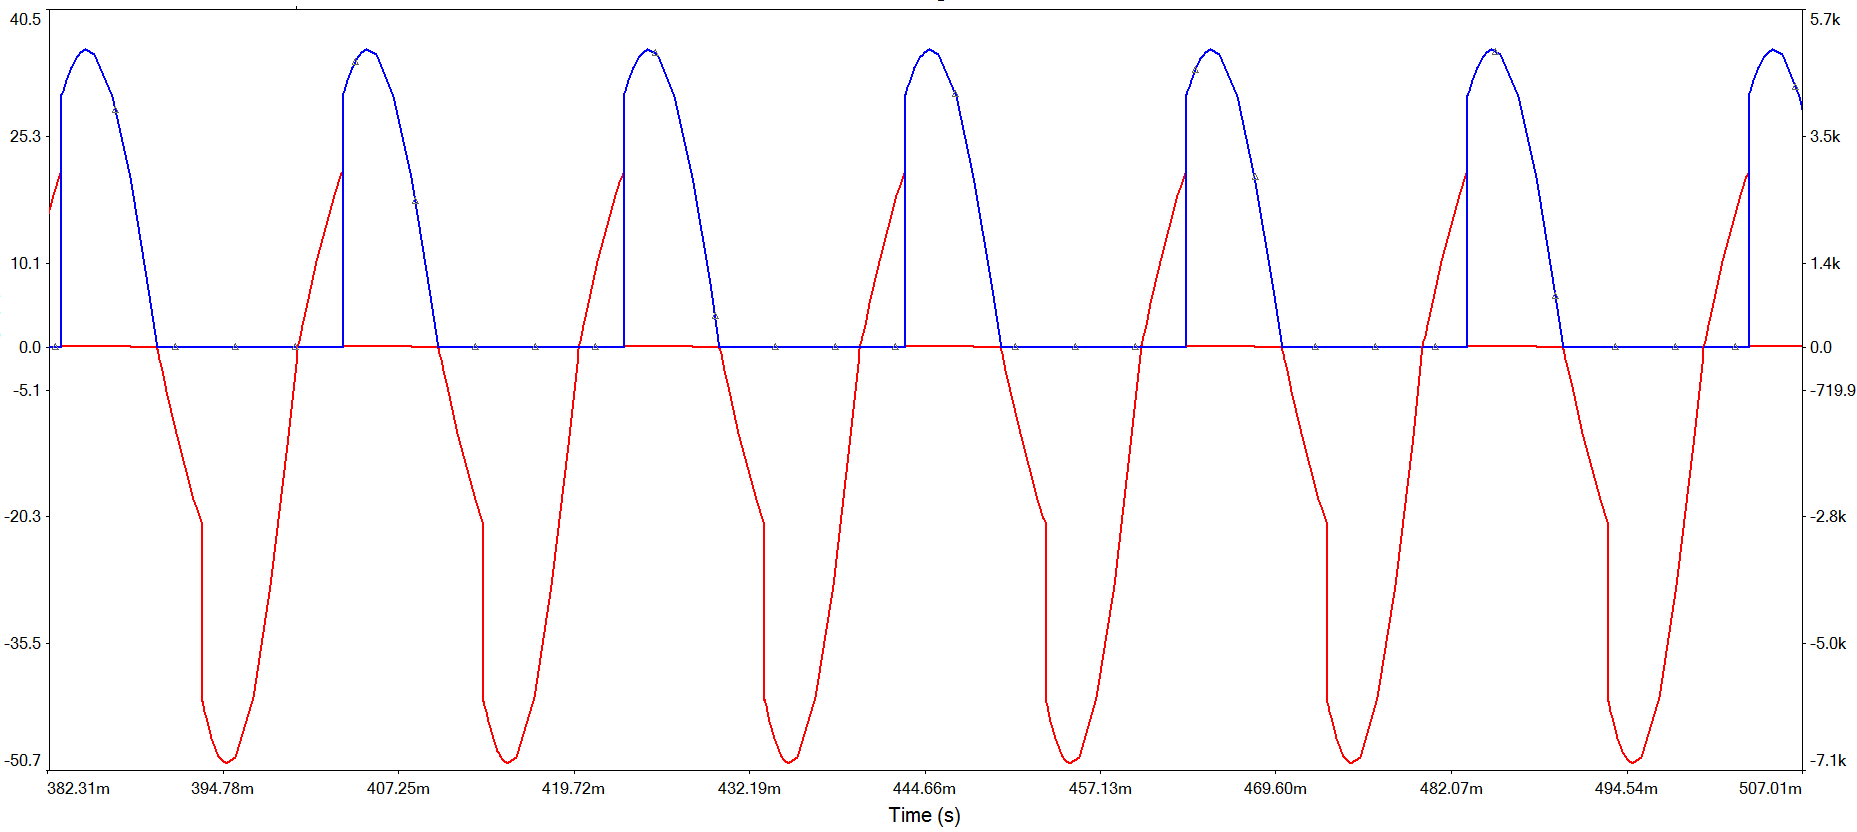
\includegraphics[keepaspectratio=true, scale=0.4]{img/circuito7}
	\caption{Tensão (sinal vermelho) e corrente (sinal azul) do tirístor.}
	\label{fig:circuit_9}
	\vspace{-0.8em}
\end{figure}

\vspace{12mm}

\subsubsection{Rectificador de onda completa com comando total e carga \textit{RL}}

De igual forma é importante visualizar o comportamento da tensão e da corrente no circuito com uma carga \textit{RL}. Os sinais à saída estão representados na \autoref{fig:circuit_10}, e para o tirístor estão representados na \autoref{fig:circuit_11}.
\pagebreak

\begin{figure}[h]
	\centering
	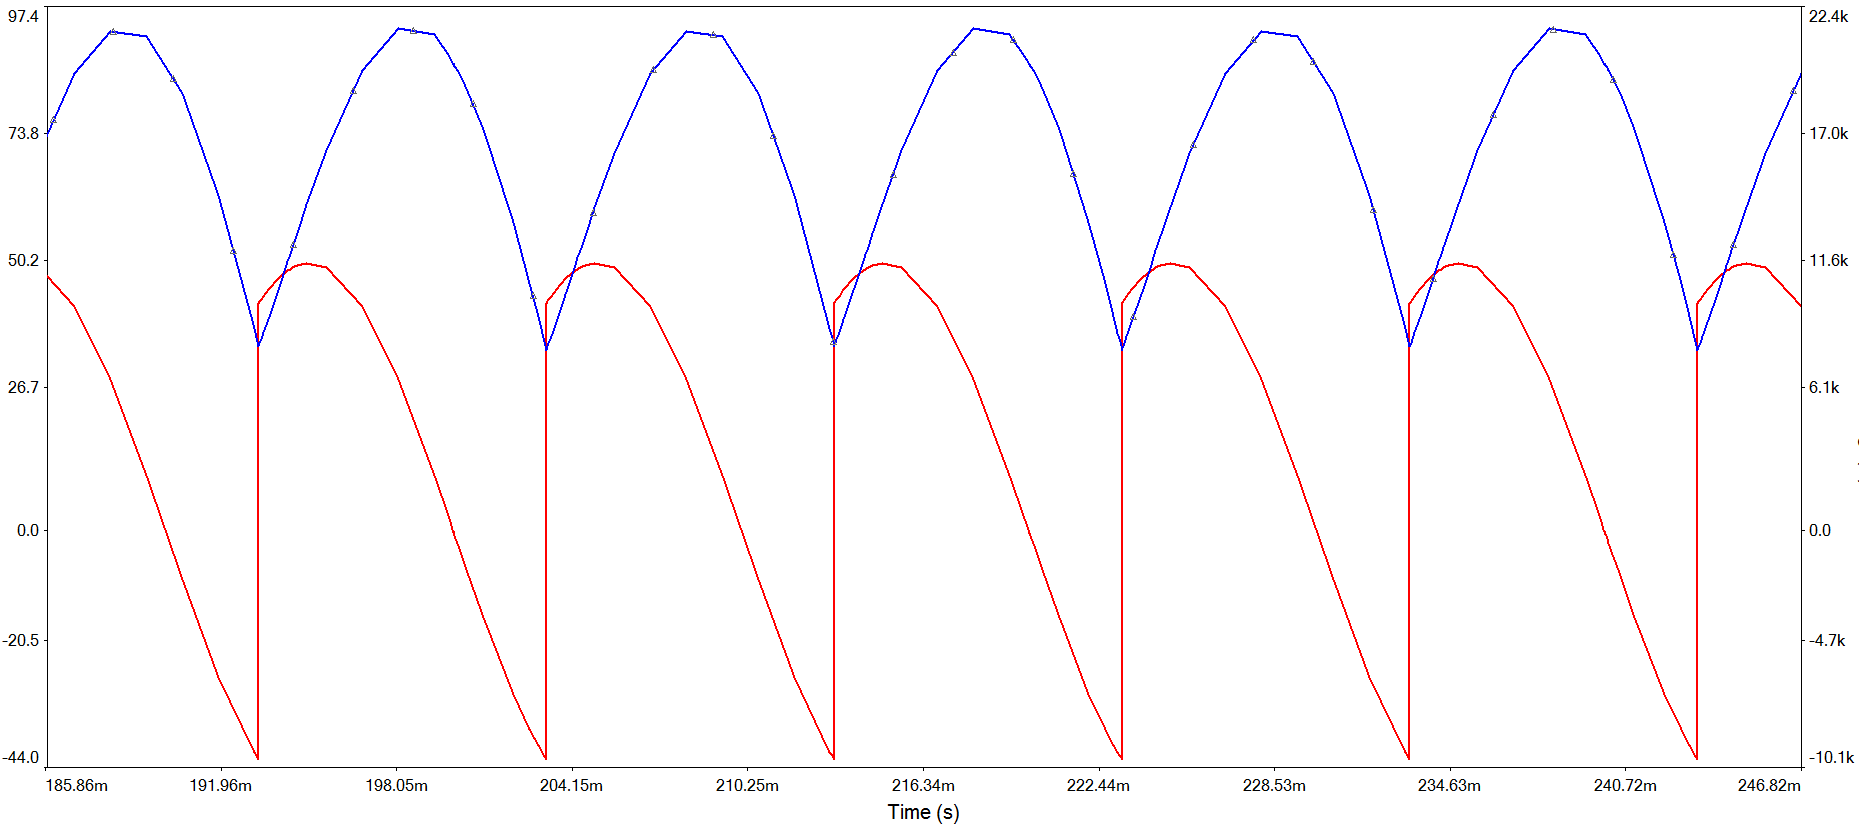
\includegraphics[keepaspectratio=true, scale=0.4]{img/circuito8}
	\caption{Tensão (sinal vermelho) e corrente (sinal azul) de saida.}
	\label{fig:circuit_10}
	\vspace{-0.8em}
\end{figure}

\begin{figure}[h]
	\centering
	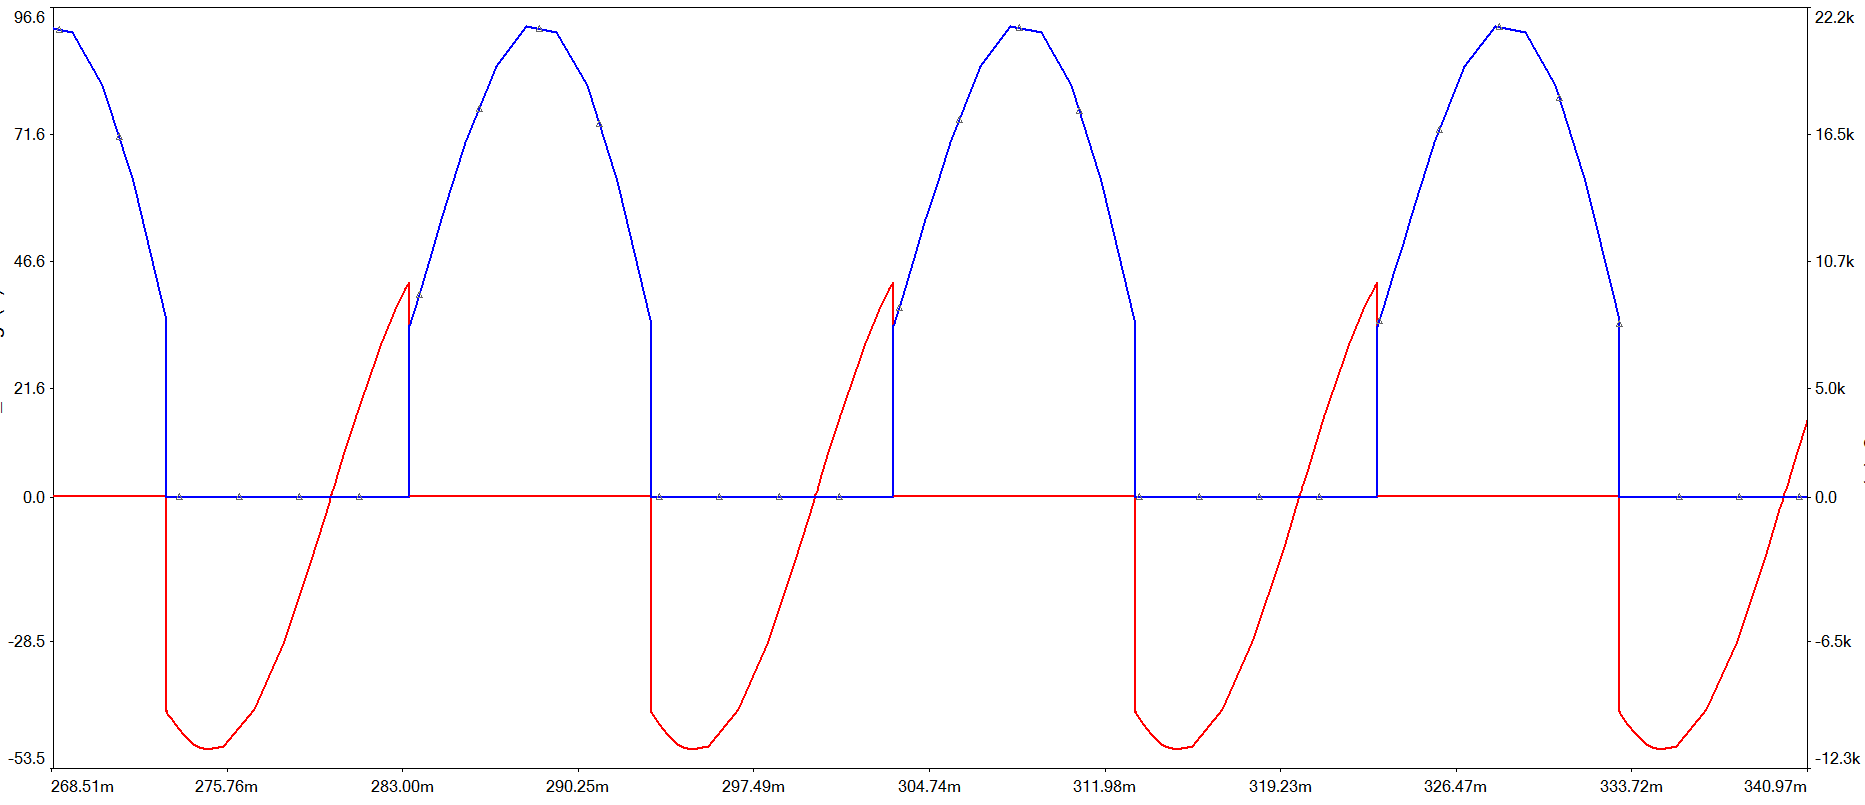
\includegraphics[keepaspectratio=true, scale=0.4]{img/circuito9}
	\caption{Tensão (sinal vermelho) e corrente (sinal azul) de tirístor.}
	\label{fig:circuit_11}
	\vspace{-0.8em}
\end{figure}

\vspace{12mm}


\subsubsection{Rectificador de onda completa semi-comandado com carga \textit{RL}}

De igual forma é importante visualizar o comportamento da tensão e da corrente no rectificador com uma carga \textit{RL} e díodos de roda livre. Os sinais à saída estão representados na \autoref{fig:circuit_12}, e no tirístor estão representados na \autoref{fig:circuit_13}.

\pagebreak
\begin{figure}[h]
	\centering
	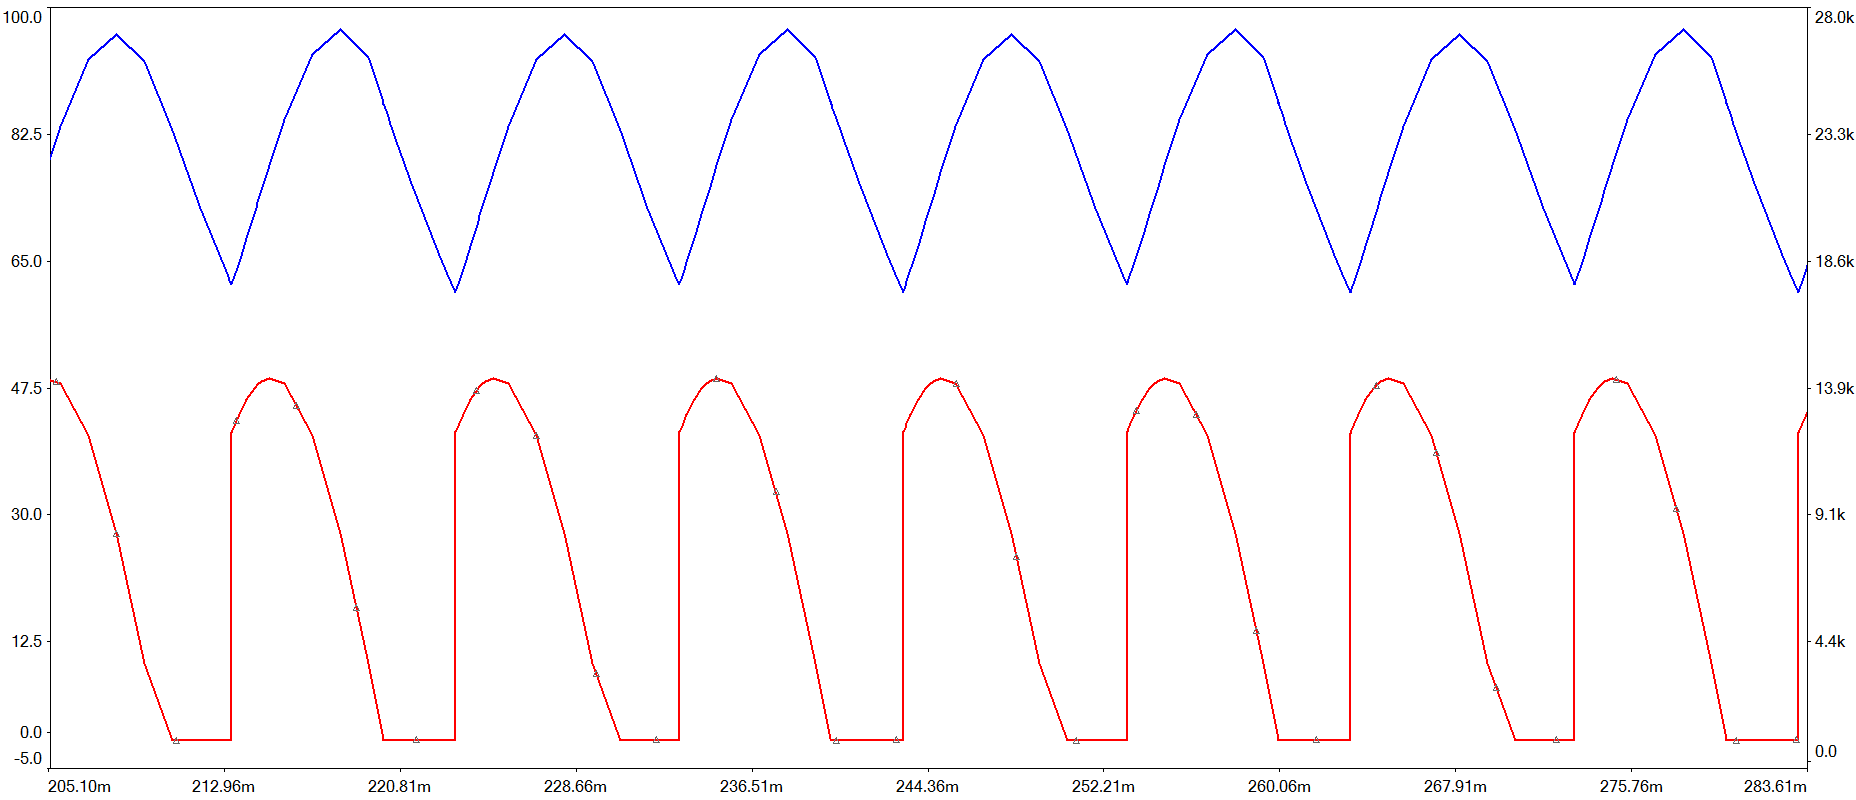
\includegraphics[keepaspectratio=true, scale=0.4]{img/circuito10}
	\caption{Tensão (sinal vermelho)e corrente (sinalazul) de saida.}
	\label{fig:circuit_12}
	\vspace{-0.8em}
\end{figure}
\vspace{15mm}
\begin{figure}[h]
	\centering
	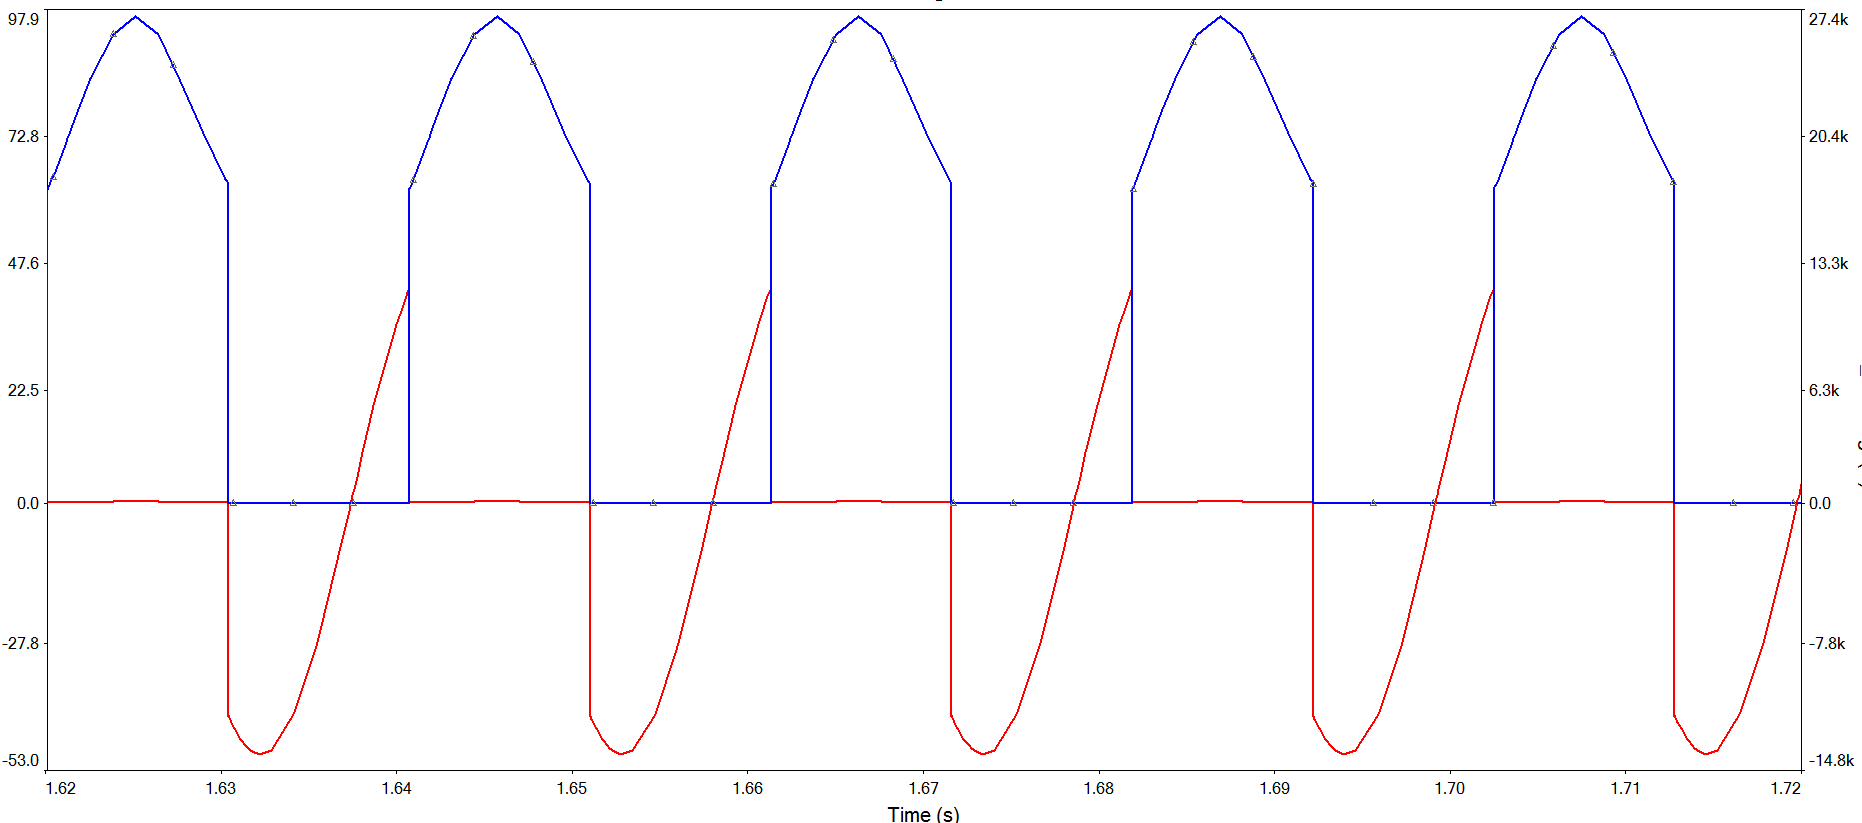
\includegraphics[keepaspectratio=true, scale=0.4]{img/circuito11}
	\caption{Tensão (sinal vermelho)e corrente (sinalazul) de tirístor.}
	\label{fig:circuit_13}
	\vspace{-0.8em}
\end{figure}


\begin{thebibliography}{2}
	
	%\bibitem{Kassakian}
	%Kassakian, John G. et al (1992, June), Principles of Power Electronics, \textit{Addison-Wesley Publishing Company}

	%\bibitem{Rashid}
	%Rashid, Muahammad H. (2004), Power Electronics - Circuits, Devices and Applications, \textit{Prentice Hall}
	
	\bibitem{Silva}
	Silva, Fernando (1998), Eletrónica Industrial, Fundação Calouste Gulbenkian
	
\end{thebibliography}


\pagebreak

\end{document}
